%%%%%%%%%%%%%%%%%%%%%%%%%%%%%%%%%%%%%%%%%
%  My documentation report
%  Objetive: Explain what I did and how, so someone can continue with the investigation
%
% Important note:
% Chapter heading images should have a 2:1 width:height ratio,
% e.g. 920px width and 460px height.
%
%%%%%%%%%%%%%%%%%%%%%%%%%%%%%%%%%%%%%%%%%

%----------------------------------------------------------------------------------------
%	PACKAGES AND OTHER DOCUMENT CONFIGURATIONS
%----------------------------------------------------------------------------------------

\documentclass[11pt,fleqn]{book} % Default font size and left-justified equations

\usepackage[top=3cm,bottom=3cm,left=3.2cm,right=3.2cm,headsep=10pt,letterpaper]{geometry} % Page margins

\usepackage{xcolor,lipsum} % Required for specifying colors by name
\definecolor{ocre}{RGB}{73,73,73} 
\definecolor{lightgray}{RGB}{229,229,229} 
% Font Settings
\usepackage{avant} % Use the Avantgarde font for headings
%\usepackage{times} % Use the Times font for headings
\usepackage{mathptmx} % Use the Adobe Times Roman as the default text font together with math symbols from the Sym­bol, Chancery and Com­puter Modern fonts

\usepackage{microtype} % Slightly tweak font spacing for aesthetics
\usepackage[utf8]{inputenc} % Required for including letters with accents
\usepackage[T1]{fontenc} % Use 8-bit encoding that has 256 glyphs


% MATHS PACKAGE
\usepackage{amsmath,tikz}
\usetikzlibrary{matrix}
\usetikzlibrary{calc}
\usetikzlibrary{shapes}
\usetikzlibrary{backgrounds,fit,shapes}
\usetikzlibrary{positioning}
\usepackage{relsize}

\newcommand*{\horzbar}{\rule[0.05ex]{2.5ex}{0.5pt}}
\usepackage{calc}

% VERBATIM PACKAGE
\usepackage{verbatim}

% Bibliography
%\usepackage[style=alphabetic,sorting=nyt,sortcites=true,autopunct=true,babel=hyphen,hyperref=true,abbreviate=false,backref=true,backend=biber]{ieeetran}

%\addbibresource{bibliography.bib} % BibTeX bibliography file
%\defbibheading{bibempty}{}

%----------------------------------------------------------------------------------------
%	VARIOUS REQUIRED PACKAGES
%----------------------------------------------------------------------------------------

\usepackage[top=3cm,bottom=3cm,left=3.2cm,right=3.2cm,headsep=10pt,letterpaper]{geometry} % Page margins

\usepackage{titlesec} % Allows customization of titles

\usepackage{graphicx} % Required for including pictures
\graphicspath{{Pictures/}} % Specifies the directory where pictures are stored

\usepackage{lipsum} % Inserts dummy text

\usepackage{tikz} % Required for drawing custom shapes

\usepackage[english]{babel} % English language/hyphenation

\usepackage{enumitem} % Customize lists
\setlist{nolistsep} % Reduce spacing between bullet points and numbered lists

\usepackage{booktabs} % Required for nicer horizontal rules in tables

\usepackage{eso-pic} % Required for specifying an image background in the title page

\usepackage{xcolor,lipsum} % Required for specifying colors by name
\definecolor{gridcal_green}{RGB}{0,170,136}
\definecolor{gridcal_green2}{RGB}{0,170,170}
%----------------------------------------------------------------------------------------
%	MAIN TABLE OF CONTENTS
%----------------------------------------------------------------------------------------

\usepackage{titletoc} % Required for manipulating the table of contents

\contentsmargin{0cm} % Removes the default margin
% Chapter text styling
\titlecontents{chapter}[1.25cm] % Indentation
{\addvspace{15pt}\large\sffamily\bfseries} % Spacing and font options for chapters
{\color{ocre!60}\contentslabel[\Large\thecontentslabel]{1.25cm}\color{ocre}} % Chapter number
{}  
{\color{ocre!60}\normalsize\sffamily\bfseries\;\titlerule*[.5pc]{.}\;\thecontentspage} % Page number
% Section text styling
\titlecontents{section}[1.25cm] % Indentation
{\addvspace{5pt}\sffamily\bfseries} % Spacing and font options for sections
{\contentslabel[\thecontentslabel]{1.25cm}} % Section number
{}
{\sffamily\hfill\color{black}\thecontentspage} % Page number
[]
% Subsection text styling
\titlecontents{subsection}[1.25cm] % Indentation
{\addvspace{1pt}\sffamily\small} % Spacing and font options for subsections
{\contentslabel[\thecontentslabel]{1.25cm}} % Subsection number
{}
{\sffamily\;\titlerule*[.5pc]{.}\;\thecontentspage} % Page number
[] 

%----------------------------------------------------------------------------------------
%	MINI TABLE OF CONTENTS IN CHAPTER HEADS
%----------------------------------------------------------------------------------------

% Section text styling
\titlecontents{lsection}[0em] % Indendating
{\footnotesize\sffamily} % Font settings
{}
{}
{}

% Subsection text styling
\titlecontents{lsubsection}[.5em] % Indentation
{\normalfont\footnotesize\sffamily} % Font settings
{}
{}
{}
 
%----------------------------------------------------------------------------------------
%	PAGE HEADERS
%----------------------------------------------------------------------------------------

\usepackage{fancyhdr} % Required for header and footer configuration

\pagestyle{fancy}
\renewcommand{\chaptermark}[1]{\markboth{\sffamily\normalsize\bfseries\chaptername\ \thechapter.\ #1}{}} % Chapter text font settings
\renewcommand{\sectionmark}[1]{\markright{\sffamily\normalsize\thesection\hspace{5pt}#1}{}} % Section text font settings
\fancyhf{} \fancyhead[LE,RO]{\sffamily\normalsize\thepage} % Font setting for the page number in the header
\fancyhead[LO]{\rightmark} % Print the nearest section name on the left side of odd pages
\fancyhead[RE]{\leftmark} % Print the current chapter name on the right side of even pages
\renewcommand{\headrulewidth}{0.5pt} % Width of the rule under the header
\addtolength{\headheight}{2.5pt} % Increase the spacing around the header slightly
\renewcommand{\footrulewidth}{0pt} % Removes the rule in the footer
\fancypagestyle{plain}{\fancyhead{}\renewcommand{\headrulewidth}{0pt}} % Style for when a plain pagestyle is specified

% Removes the header from odd empty pages at the end of chapters
\makeatletter
\renewcommand{\cleardoublepage}{
\clearpage\ifodd\c@page\else
\hbox{}
\vspace*{\fill}
\thispagestyle{empty}
\newpage
\fi}

%----------------------------------------------------------------------------------------
%	THEOREM STYLES
%----------------------------------------------------------------------------------------

\usepackage{amsmath,amsfonts,amssymb,amsthm} % For math equations, theorems, symbols, etc

\newcommand{\intoo}[2]{\mathopen{]}#1\,;#2\mathclose{[}}
\newcommand{\ud}{\mathop{\mathrm{{}d}}\mathopen{}}
\newcommand{\intff}[2]{\mathopen{[}#1\,;#2\mathclose{]}}
\newtheorem{notation}{Notation}[chapter]

%%%%%%%%%%%%%%%%%%%%%%%%%%%%%%%%%%%%%%%%%%%%%%%%%%%%%%%%%%%%%%%%%%%%%%%%%%%
%%%%%%%%%%%%%%%%%%%% dedicated to boxed/framed environements %%%%%%%%%%%%%%
%%%%%%%%%%%%%%%%%%%%%%%%%%%%%%%%%%%%%%%%%%%%%%%%%%%%%%%%%%%%%%%%%%%%%%%%%%%
\newtheoremstyle{ocrenumbox}% % Theorem style name
{0pt}% Space above
{0pt}% Space below
{\normalfont}% % Body font
{}% Indent amount
{\small\bf\sffamily\color{ocre}}% % Theorem head font
{\;}% Punctuation after theorem head
{0.25em}% Space after theorem head
{\small\sffamily\color{ocre}\thmname{#1}\nobreakspace\thmnumber{\@ifnotempty{#1}{}\@upn{#2}}% Theorem text (e.g. Theorem 2.1)
\thmnote{\nobreakspace\the\thm@notefont\sffamily\bfseries\color{black}---\nobreakspace#3.}} % Optional theorem note
\renewcommand{\qedsymbol}{$\blacksquare$}% Optional qed square

\newtheoremstyle{blacknumex}% Theorem style name
{5pt}% Space above
{5pt}% Space below
{\normalfont}% Body font
{} % Indent amount
{\small\bf\sffamily}% Theorem head font
{\;}% Punctuation after theorem head
{0.25em}% Space after theorem head
{\small\sffamily{\tiny\ensuremath{\blacksquare}}\nobreakspace\thmname{#1}\nobreakspace\thmnumber{\@ifnotempty{#1}{}\@upn{#2}}% Theorem text (e.g. Theorem 2.1)
\thmnote{\nobreakspace\the\thm@notefont\sffamily\bfseries---\nobreakspace#3.}}% Optional theorem note

\newtheoremstyle{blacknumbox} % Theorem style name
{0pt}% Space above
{0pt}% Space below
{\normalfont}% Body font
{}% Indent amount
{\small\bf\sffamily}% Theorem head font
{\;}% Punctuation after theorem head
{0.25em}% Space after theorem head
{\small\sffamily\thmname{#1}\nobreakspace\thmnumber{\@ifnotempty{#1}{}\@upn{#2}}% Theorem text (e.g. Theorem 2.1)
\thmnote{\nobreakspace\the\thm@notefont\sffamily\bfseries---\nobreakspace#3.}}% Optional theorem note

%%%%%%%%%%%%%%%%%%%%%%%%%%%%%%%%%%%%%%%%%%%%%%%%%%%%%%%%%%%%%%%%%%%%%%%%%%%
%%%%%%%%%%%%% dedicated to non-boxed/non-framed environements %%%%%%%%%%%%%
%%%%%%%%%%%%%%%%%%%%%%%%%%%%%%%%%%%%%%%%%%%%%%%%%%%%%%%%%%%%%%%%%%%%%%%%%%%
\newtheoremstyle{ocrenum}% % Theorem style name
{5pt}% Space above
{5pt}% Space below
{\normalfont}% % Body font
{}% Indent amount
{\small\bf\sffamily\color{ocre}}% % Theorem head font
{\;}% Punctuation after theorem head
{0.25em}% Space after theorem head
{\small\sffamily\color{ocre}\thmname{#1}\nobreakspace\thmnumber{\@ifnotempty{#1}{}\@upn{#2}}% Theorem text (e.g. Theorem 2.1)
\thmnote{\nobreakspace\the\thm@notefont\sffamily\bfseries\color{black}---\nobreakspace#3.}} % Optional theorem note
\renewcommand{\qedsymbol}{$\blacksquare$}% Optional qed square
\makeatother

% Defines the theorem text style for each type of theorem to one of the three styles above
\newcounter{dummy} 
\numberwithin{dummy}{section}
\theoremstyle{ocrenumbox}
\newtheorem{theoremeT}[dummy]{Theorem}
\newtheorem{problem}{Problem}[chapter]
\newtheorem{exerciseT}{Exercise}[chapter]
\theoremstyle{blacknumex}
\newtheorem{exampleT}{Example}[chapter]
\theoremstyle{blacknumbox}
\newtheorem{vocabulary}{Vocabulary}[chapter]
\newtheorem{definitionT}{Definition}[section]
\newtheorem{corollaryT}[dummy]{Corollary}
\theoremstyle{ocrenum}
\newtheorem{proposition}[dummy]{Proposition}

%----------------------------------------------------------------------------------------
%	DEFINITION OF COLORED BOXES
%----------------------------------------------------------------------------------------

\RequirePackage[framemethod=default]{mdframed} % Required for creating the theorem, definition, exercise and corollary boxes

% Theorem box
\newmdenv[skipabove=7pt,
skipbelow=7pt,
backgroundcolor=black!5,
linecolor=ocre,
innerleftmargin=5pt,
innerrightmargin=5pt,
innertopmargin=5pt,
leftmargin=0cm,
rightmargin=0cm,
innerbottommargin=5pt]{tBox}

% Exercise box	  
\newmdenv[skipabove=7pt,
skipbelow=7pt,
rightline=false,
leftline=true,
topline=false,
bottomline=false,
backgroundcolor=ocre!10,
linecolor=ocre,
innerleftmargin=5pt,
innerrightmargin=5pt,
innertopmargin=5pt,
innerbottommargin=5pt,
leftmargin=0cm,
rightmargin=0cm,
linewidth=4pt]{eBox}	

% Definition box
\newmdenv[skipabove=7pt,
skipbelow=7pt,
rightline=false,
leftline=true,
topline=false,
bottomline=false,
linecolor=ocre,
innerleftmargin=5pt,
innerrightmargin=5pt,
innertopmargin=0pt,
leftmargin=0cm,
rightmargin=0cm,
linewidth=4pt,
innerbottommargin=0pt]{dBox}	

% Corollary box
\newmdenv[skipabove=7pt,
skipbelow=7pt,
rightline=false,
leftline=true,
topline=false,
bottomline=false,
linecolor=gray,
backgroundcolor=black!5,
innerleftmargin=5pt,
innerrightmargin=5pt,
innertopmargin=5pt,
leftmargin=0cm,
rightmargin=0cm,
linewidth=4pt,
innerbottommargin=5pt]{cBox}

% Creates an environment for each type of theorem and assigns it a theorem text style from the "Theorem Styles" section above and a colored box from above
\newenvironment{theorem}{\begin{tBox}\begin{theoremeT}}{\end{theoremeT}\end{tBox}}
\newenvironment{exercise}{\begin{eBox}\begin{exerciseT}}{\hfill{\color{ocre}\tiny\ensuremath{\blacksquare}}\end{exerciseT}\end{eBox}}				  
\newenvironment{definition}{\begin{dBox}\begin{definitionT}}{\end{definitionT}\end{dBox}}	
\newenvironment{example}{\begin{exampleT}}{\hfill{\tiny\ensuremath{\blacksquare}}\end{exampleT}}		
\newenvironment{corollary}{\begin{cBox}\begin{corollaryT}}{\end{corollaryT}\end{cBox}}	

%----------------------------------------------------------------------------------------
%	REMARK ENVIRONMENT
%----------------------------------------------------------------------------------------

\newenvironment{remark}{\par\vspace{10pt}\small % Vertical white space above the remark and smaller font size
\begin{list}{}{
\leftmargin=35pt % Indentation on the left
\rightmargin=25pt}\item\ignorespaces % Indentation on the right
\makebox[-2.5pt]{\begin{tikzpicture}[overlay]
\node[draw=ocre!60,line width=1pt,circle,fill=ocre!25,font=\sffamily\bfseries,inner sep=2pt,outer sep=0pt] at (-15pt,0pt){\textcolor{ocre}{R}};\end{tikzpicture}} % Orange R in a circle
\advance\baselineskip -1pt}{\end{list}\vskip5pt} % Tighter line spacing and white space after remark

%----------------------------------------------------------------------------------------
%	SECTION NUMBERING IN THE MARGIN
%----------------------------------------------------------------------------------------

\makeatletter
\renewcommand{\@seccntformat}[1]{\llap{\textcolor{ocre}{\csname the#1\endcsname}\hspace{1em}}}                    
\renewcommand{\section}{\@startsection{section}{1}{\z@}
{-4ex \@plus -1ex \@minus -.4ex}
{1ex \@plus.2ex }
{\normalfont\large\sffamily\bfseries}}
\renewcommand{\subsection}{\@startsection {subsection}{2}{\z@}
{-3ex \@plus -0.1ex \@minus -.4ex}
{0.5ex \@plus.2ex }
{\normalfont\sffamily\bfseries}}
\renewcommand{\subsubsection}{\@startsection {subsubsection}{3}{\z@}
{-2ex \@plus -0.1ex \@minus -.2ex}
{.2ex \@plus.2ex }
{\normalfont\small\sffamily\bfseries}}                        
\renewcommand\paragraph{\@startsection{paragraph}{4}{\z@}
{-2ex \@plus-.2ex \@minus .2ex}
{.1ex}
{\normalfont\small\sffamily\bfseries}}

%----------------------------------------------------------------------------------------
%	HYPERLINKS IN THE DOCUMENTS
%----------------------------------------------------------------------------------------

% For an unclear reason, the package should be loaded now and not later
\usepackage{hyperref}
\hypersetup{hidelinks,backref=true,pagebackref=true,hyperindex=true,colorlinks=false,breaklinks=true,urlcolor= ocre,bookmarks=true,bookmarksopen=false,pdftitle={Title},pdfauthor={Author}}

%----------------------------------------------------------------------------------------
%	CHAPTER HEADINGS
%----------------------------------------------------------------------------------------

% The set-up below should be (sadly) manually adapted to the overall margin page septup controlled by the geometry package loaded in the main.tex document. It is possible to implement below the dimensions used in the goemetry package (top,bottom,left,right)... TO BE DONE

% Command to use pictures
\newcommand{\thechapterimage}{}
\newcommand{\chapterimage}{}

% Numbered chapters with mini tableofcontents
\def\thechapter{\arabic{chapter}}
\def\@makechapterhead#1{
	\thispagestyle{empty}
	{\centering \normalfont\sffamily
		\ifnum \c@secnumdepth >\m@ne
		\if@mainmatter
		\startcontents
		\begin{tikzpicture}[remember picture,overlay]
		\node at (current page.north west)
		{\begin{tikzpicture}[remember picture,overlay]
%			\node[anchor=north west,inner sep=0pt] at (0,0) {\includegraphics[width=\paperwidth]{\thechapterimage}};
%			\fill[gridcal_green] (-50mm,250mm) rectangle (180mm,200mm)
%%%%%%%%%%%%%%%%%%%%%%%%%%%%%%%%%%%%%%%%%%%%%%%%%%%%%%%%%%%%%%%%%%%%%%%%%%%%%%%%%%%%%
% Commenting the 3 lines below removes the small contents box in the chapter heading
%\fill[color=ocre!10!white,opacity=.6] (1cm,0) rectangle (8cm,-7cm);
%\node[anchor=north west] at (1.1cm,.35cm) {\parbox[t][8cm][t]{6.5cm}{\huge\bfseries\flushleft \printcontents{l}{1}{\setcounter{tocdepth}{2}}}};
\draw[anchor=west] (5cm,-9cm) node [rounded corners=20pt,fill=ocre!10!white,text opacity=1,draw=ocre,draw opacity=1,line width=1.5pt,fill opacity=.6,inner sep=12pt]{\huge\sffamily\bfseries\textcolor{black}{\thechapter. #1\strut\makebox[22cm]{}}};
%%%%%%%%%%%%%%%%%%%%%%%%%%%%%%%%%%%%%%%%%%%%%%%%%%%%%%%%%%%%%%%%%%%%%%%%%%%%%%%%%%%%%
\end{tikzpicture}};
\end{tikzpicture}}
\par\vspace*{230\p@}
\fi
\fi}

%%%%%%%%%%%%%%%%%%%%%%%%%%%%%%%%%%%%%%%%%%%%%%%%%%%%%%%%%%%%%%%%%%%%%%%%%%%%%%%%%%%%%
%%%%%%%%%%%%%%%%%%%%%%%%%%%%%%%%%%%%%%%%%%%%%%%%%%%%%%%%%%%%%%%%%%%%%%%%%%%%%%%%%%%%%
%\newcommand{\chapterbox}[1]{}
%
%% Numbered chapters with mini tableofcontents
%\def\thechapter{\arabic{chapter}}
%\def\@makechapterhead#1{
%	\thispagestyle{empty}
%	{\centering \normalfont\sffamily
%		\ifnum \c@secnumdepth >\m@ne
%		\if@mainmatter
%		\startcontents
%		\begin{tikzpicture}[remember picture,overlay]
%		\node at (current page.north west)
%		{\begin{tikzpicture}[remember picture,overlay]
%			\shade[top color=gridcal_green,bottom color=gridcal_green2] (-50mm,250mm) rectangle (180mm,200mm)
%		};
%%%%%%%%%%%%%%%%%%%%%%%%%%%%%%%%%%%%%%%%%%%%%%%%%%%%%%%%%%%%%%%%%%%%%%%%%%%%%%%%%%%%%%
%% Commenting the 3 lines below removes the small contents box in the chapter heading
%%\fill[color=ocre!10!white,opacity=.6] (1cm,0) rectangle (8cm,-7cm);
%%\node[anchor=north west] at (1.1cm,.35cm) {\parbox[t][8cm][t]{6.5cm}{\huge\bfseries\flushleft \printcontents{l}{1}{\setcounter{tocdepth}{2}}}};
%\draw[anchor=west] (5cm,-9cm) node [rounded corners=20pt,fill=ocre!10!white,text opacity=1,draw=ocre,draw opacity=1,line width=1.5pt,fill opacity=.6,inner sep=12pt]{\huge\sffamily\bfseries\textcolor{black}{\thechapter. #1\strut\makebox[22cm]{}}};
%%%%%%%%%%%%%%%%%%%%%%%%%%%%%%%%%%%%%%%%%%%%%%%%%%%%%%%%%%%%%%%%%%%%%%%%%%%%%%%%%%%%%%
%\end{tikzpicture}};




% Unnumbered chapters without mini tableofcontents (could be added though) 
\def\@makeschapterhead#1{
\thispagestyle{empty}
{\centering \normalfont\sffamily
\ifnum \c@secnumdepth >\m@ne
\if@mainmatter
\begin{tikzpicture}[remember picture,overlay]
\node at (current page.north west)
{\begin{tikzpicture}[remember picture,overlay]
\node[anchor=north west,inner sep=0pt] at (0,0) {\includegraphics[width=\paperwidth]{\thechapterimage}};
\draw[anchor=west] (5cm,-9cm) node [rounded corners=20pt,fill=ocre!10!white,fill opacity=.6,inner sep=12pt,text opacity=1,draw=ocre,draw opacity=1,line width=1.5pt]{\huge\sffamily\bfseries\textcolor{black}{#1\strut\makebox[22cm]{}}};
\end{tikzpicture}};
\end{tikzpicture}}
\par\vspace*{230\p@}
\fi
\fi
}
\makeatother % Insert the commands.tex file which contains the majority of the structure behind the template

\begin{document}

\let\cleardoublepage\clearpage

%----------------------------------------------------------------------------------------
%	TITLE PAGE
%----------------------------------------------------------------------------------------

\begingroup
\thispagestyle{empty}

\AddToShipoutPicture*{\put(0,0){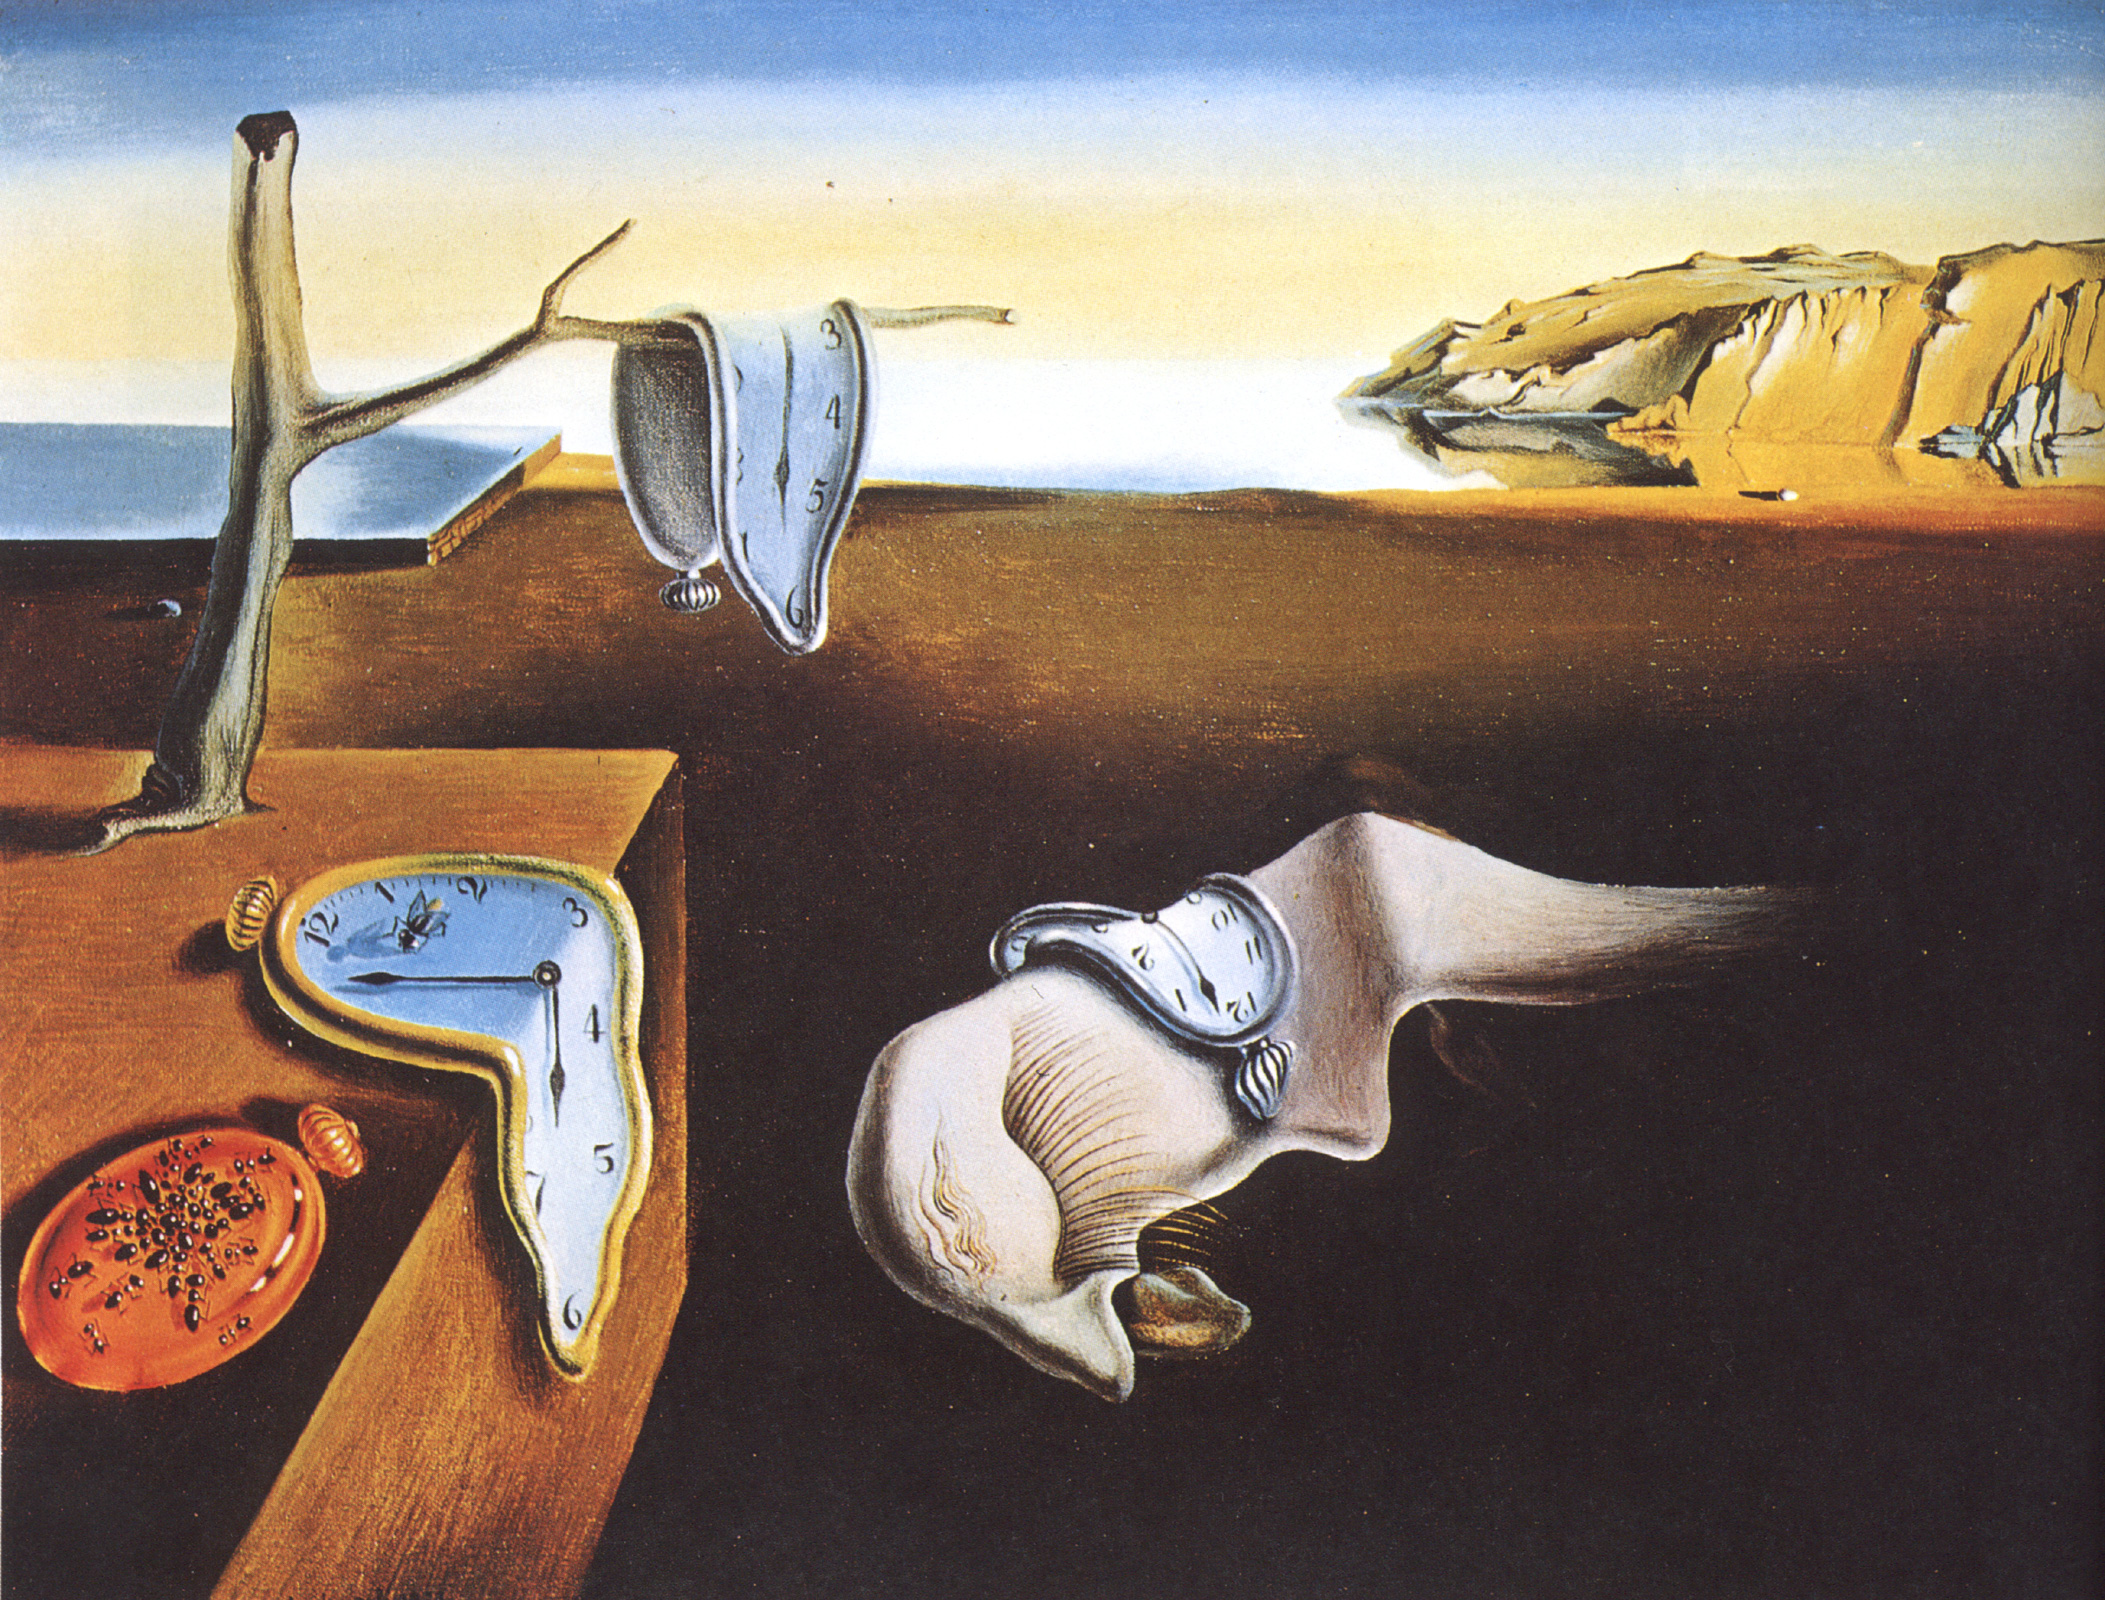
\includegraphics[scale=4.2]{frontpage}}} % Image background

\begin{tikzpicture}[remember picture, overlay]
\node[fill=white, fill opacity=0.6, anchor=north,minimum height=6cm, minimum width=\paperwidth] (names) at ([yshift=19cm]current page.south){};
\node[font=\normalfont\fontsize{35}{35}\sffamily\selectfont] at ([yshift=17cm]current page.south) {GridCal};
\node[font=\normalfont\fontsize{35}{35}\sffamily\selectfont \Huge] at ([yshift=15cm]current page.south) {Santiago Peñate Vera};
\end{tikzpicture}



%\centering
%%\vspace{5cm}
%\par\normalfont\fontsize{35}{35}\sffamily\selectfont
%\textbf{GridCal Manual }\\
%{\LARGE }\par % Book title
%\vspace*{1cm}
%{\Huge Santiago Peñate Vera}\par % Author name
%\endgroup

%----------------------------------------------------------------------------------------
%	COPYRIGHT PAGE
%----------------------------------------------------------------------------------------

\newpage
~\vfill
\thispagestyle{empty}

%\noindent Copyright \copyright\ 2014 Andrea Hidalgo\\ % Copyright notice

\noindent \textsc{GridCal}\\

\noindent Research oriented power systems software.\\ % License information

\noindent \textit{Started writing this document in Madrid the 9th of October of 2016} % Printing/edition date

%----------------------------------------------------------------------------------------
%	TABLE OF CONTENTS
%----------------------------------------------------------------------------------------

\chapterimage{chapterhdr1.jpg} % heading image

\pagestyle{empty} % No headers

\renewcommand\contentsname{Table of content}
%\renewcommand{\bibname}{Bibliography}
\tableofcontents% Print the table of contents itself

%\cleardoublepage % Forces the first chapter to start on an odd page so it's on the right

\pagestyle{fancy} % Print headers again

%----------------------------------------------------------------------------------------
%	CHAPTER 1
%----------------------------------------------------------------------------------------

\chapterimage{chapterhdr1.jpg} % Chapter heading image

\chapter{Introduction}

GridCal is a research oriented power systems software.  \newline

Research oriented? How? Well, it is a fruit of research. It is designed to be modular. As a researcher I found that the available software (not even talking about commercial options) are hard to expand or adapt to achieve complex simulations. GridCal is designed to allow you to build and reuse modules, which eventually will boost your productivity and the possibilities that are at hand. \newline

I have made other projects (even another open source one: fPotencia in C++). I believe that this project encapsulates my half life of programming experience and the curiosity I have developed for power systems. \newline

So, I do really hope you enjoy it, and if you have comments, suggestions or just want to collaborate, do not hesitate to contact.\newline

\begin{flushright}
	Cheers, 

Santiago
\end{flushright}

\newpage
\section{installation}


GridCal is designed to work with python 3.5 and onwards, hence retro-compatibility is not guaranteed.

\subsection{Windows}

Open a system console (go to the desktop menu and type \verb|cmd|, the console should appear). Then type:\newline

\verb|pip install GridCal| \newline

This assumes that your system-wide python is a python 3 distribution, hence you must make sure of this. An easy way to check this, is to open a console, type \verb|python| and if a python 3 console opens within the terminal, then it is allright.

For windows systems I have disabled the installation of PyQt (the user interface technology) because it conflicts with the Qt version provided by Anaconda. This should not be the case, but it happens. Therefore, under windows, you must install python through Anaconda.

\subsection{Linux / OSX}

On Unix systems the python 2 / 3 issue is non existent since the terminal commands for python 2 and python 3 are different. So, simply go to a system terminal and type:\newline

\verb|pip3 install GridCal|  \newline

This command will install all the dependencies flawlessly unlike under windows.


\section{Run with user interface}

You must have Python 3.5 or higher installed to work with the GUI. From a Python console:

\begin{verbatim}
from GridCal.ExecuteGridCal import run
run()
\end{verbatim}

\subsection{Windows}

To run GridCal with GUI directly from a system console, type:\newline

\verb|python -c "from GridCal.ExecuteGridCal import run; run()"|\newline

You can embed this command in a shortcut file, and have a windows shortcut in the desktop for GridCal.

\subsection{Linux / OSX}

To run GridCal with GUI directly from a system console, type:\newline

\verb|python3 -c "from GridCal.ExecuteGridCal import run; run()"|\newline



\section{Using GridCal as a library}

You can use the calculation engine directly or from other applications: \newline

\verb|from GridCal.Engine.CalculationEngine import *| \newline

This will provide access to all the objects in the calculation engine of GridCal.


%----------------------------------------------------------------------------------------
%	CHAPTER 2
%----------------------------------------------------------------------------------------

\chapterimage{chapterhdr1.jpg} % Chapter heading image
\chapter{Structure}

GridCal uses an object oriented approach for all the data and simulation management. However the object orientation is very inefficient when used in numerical computation, that is why there are \verb|compile()| functions that extract the information out of the objects and turn this information into vectors, matrices and DataFrames in order to have efficient numerical computations. After having been involved in quite some number-crunching software developments, I have found this approach to be the best compromise between efficiency and code escalability and maintainability .

The whole idea can be summarized as:

\begin{verbatim}
Object oriented structures -> intermediate objects holding arrays -> Numerical modules
\end{verbatim}




\section{Circuit and MultiCircuit}

The concept of circuit should be easy enough to understand. It represents a set of nodes (buses) and branches (lines, transformers or other impedances)


The \verb|MultiCircuit| class is the main object in GridCal. It represents a circuit that may contain islands. It is important to understand that a circuit split in two or more islands cannot be simulated as is, because the admittance matrix would be singular. The solution to this is to split the circuit in island-circuits. Therefore \verb|MultiCircuit| identifies the islands and creates individual \verb|Circuit| objects for each of them.

As I said before GridCal uses an object oriented approach for the data management. This allows to group the data in a smart way. In GridCal I have decided to have only two types of object directly declared in a \verb|Circuit| or \verb|MultiCircuit| object. These are the \verb|Bus| and the \verb|Branch|. The branches connect the buses and the buses contain all the other possible devices like loads, generators, batteries, etc. This simplifies enormously the management of element when adding, associating and deleting.

\subsection{Circuit}

\begin{itemize}
	\item $Sbase$: Base power to compute the per unit power values (MVA)
	\item $branch\_original\_idx$: Array that keeps the index of the branches in the parent MultiCircuit object.
	\item $branches$: List of Branch objects.
	\item $bus\_original\_idx$: Array that keeps the index of the buses in the parent MultiCircuit object.
	\item $buses$: List of Bus objects.
	\item $graph$: Graph object from the \verb|networkx| package.
	\item $mc\_time\_series$
	\item $monte\_carlo\_input$
	\item $name$: Name of the circuit.
	\item $power\_flow\_input$
	\item $power\_flow\_results$
	\item $time\_series\_input$
	\item $time\_series\_results$
\end{itemize}


\subsection{MultiCircuit (inherits Circuit)}

Since the MultiCircuit inherits the Circuit object, it means that it has by default all the properties of the Circuit plus the ones that are below.

\begin{itemize}
	\item $branch\_dictionary$
	\item $branch\_names$: Array with the name of the branch objects all together.
	\item $bus\_dictionary$
	\item $bus\_names$: Array with the name of the bus objects all together.
	\item $circuits$: List of the Circuit objects. Each Circuit represents an island.
	\item $has\_time\_series$: Are there time series available? (True/False)
\end{itemize}


\section{Bus object}

The Bus object is the container of all the possible devices that can be attached to a bus bar or substation. Such objects can be loads, voltage controlled generators, static generators, batteries, shunt elements, etc.

\begin{itemize}
	\item $Qmax\_sum$: Maximum reactive power of this bus (inferred from the devices).
	\item $Qmin\_sum$: Minimum reactive power of this bus (inferred from the devices).
	\item $Vmax$: Maximum voltage of this bus (p.u.)
	\item $Vmin$: Minimum voltage of this bus (p.u.)
	\item $Vnom$: Nominal voltage of the bus (kV)
	\item $batteries$: List of Battery objects.
	\item $controlled\_generators$: List of ControlledGenerator objects.
	\item $dispatch\_storage$: Shall this bus dispatch its storage devices?  (True / False)
	\item $graphic\_object$: Qt graphic object associated to this bus.
	\item $is\_enabled$: Is this bus enabled for calculation? (True / False)
	\item $is\_slack$: Is this bus a slack bus? (True / False)
	\item $loads$: List of Load objects.
	\item $name$: Name of the element.
	\item $shunts$: List of Shunt objects.
	\item $static\_generators$: List of StaticGenerator objects.
	\item $type$: Type of the bus.
	\item $x$: x coordinate of the bus for representation.
	\item $y$: y coordinate of the bus for representation.
\end{itemize}


\subsection{Load object}

The load object implements the so-called ZIP model, in which the load can be represented by a combination of power (P), current(I), and impedance (Z).

\begin{itemize}
	\item $I$: Current (complex, in kA)
	\item $Iprof$: Pandas DataFrame with the current profile (complex, in kA)
	\item $S$: Power (complex in MVA)
	\item $Sprof$: Pandas DataFrame with the power profile (complex, in MVA)
	\item $Z$: Impedance (complex, in Ohm)
	\item $Zprof$: Pandas DataFrame with the impedance profile (complex, in Ohm)
	\item $name$: Name of the load.
\end{itemize}

The sign convention is: Positive to act as a load, negative to act as a generator.

\subsection{StaticGenerator object}

\begin{itemize}
	\item $S$: Power (complex in MVA)
	\item $Sprof$ Pandas DataFrame with the power profile (complex, in MVA)
	\item $name$: Name of the StaticGenerator.
\end{itemize}




\subsection{Battery object}

\begin{itemize}
	\item $Enom$: Nominal energy capacity (MWh)
	\item $P$: Active power being dispatched (MW)
	\item $Pprof$: Pandas DataFrame with the active power profile (real, in MW)
	\item $Qmax$: reactive power upper limit (p.u.)
	\item $Qmin$: reactive power lower limit (p.u.)
	\item $Snom$: Nominal power (MVA)
	\item $Vset$: Voltage set point (p.u.)
	\item $Vset\_prof$ Pandas DataFrame with the voltage set point profile (p.u.)
	\item $name$: Name of the battery.
\end{itemize}



\subsection{ControlledGenerator object}

\begin{itemize}
	\item $P$: Active power being dispatched (MW)
	\item $Pprof$: Pandas DataFrame with the active power profile (real, in MW)
	\item $Qmax$: reactive power upper limit (p.u.)
	\item $Qmin$: reactive power lower limit (p.u.)
	\item $Snom$: Nominal power (MVA)
	\item $Vset$: Voltage set point (p.u.)
	\item $Vset\_prof$ Pandas DataFrame with the voltage set point profile (p.u.)
	\item $name$: Name of the ControlledGenerator.
\end{itemize}



\subsection{Shunt object}

\begin{itemize}
	\item $Y$: Admittance of the shunt object (in p.u.)
	\item $Yprof$: Pandas DataFrame with the admittance profile (p.u.)
	\item $name$: Name of the shunt object.
\end{itemize}



\section{Branch object}


\begin{itemize}
	\item $angle$: Tap angle in radians.
	\item $bus_from$: Bus object to which the branch is connected at the "from" end.
	\item $bus_to$: Bus object to which the branch is connected at the "to" end.
	\item $is\_enabled$: Is this branch enabled for calculation?
	\item $mttf$: Mean time to failure (h)
	\item $mttr$: Mean time to repair (h)
	\item $name$: Name of the branch
	\item $rate$: Power rating (MVA)
	\item $tap\_module$: tap changer module (value around 1)
	\item $y\_shunt$: Total shunt admittance.
	\item $z\_series$: Total series impedance.
	\item $type\_obj$: Object of type TransformerType or LineType used to set the current impedance values. \newline
\end{itemize}

Implements the model at \ref{Universal_branch_model}.



\section{TransformerType object}

\begin{itemize}
	\item $HV\_nominal\_voltage$: High voltage side nominal voltage (kV)
	\item $LV\_nominal\_voltage$: Low voltage side nominal voltage (kV)
	\item $Nominal\_power$: Transformer nominal power (MVA)
	\item $Copper\_losses$: Copper losses (kW)
	\item $Iron\_losses$: Iron Losses (kW)
	\item $No\_load\_current$: No load current (\%)
	\item $Short\_circuit\_voltage$: Short circuit voltage (\%)
	\item $GR\_hv1$:
	\item $GX\_hv1$:  \newline
\end{itemize}

Implements the model at \ref{Transformer_definition}.



\section{Class diagram}

Here the API class diagram is sketched. All the classes are included but only the most fundamental properties and functions od each class are included to keep the diagram simple.

\begin{figure}[h]
	\centering
	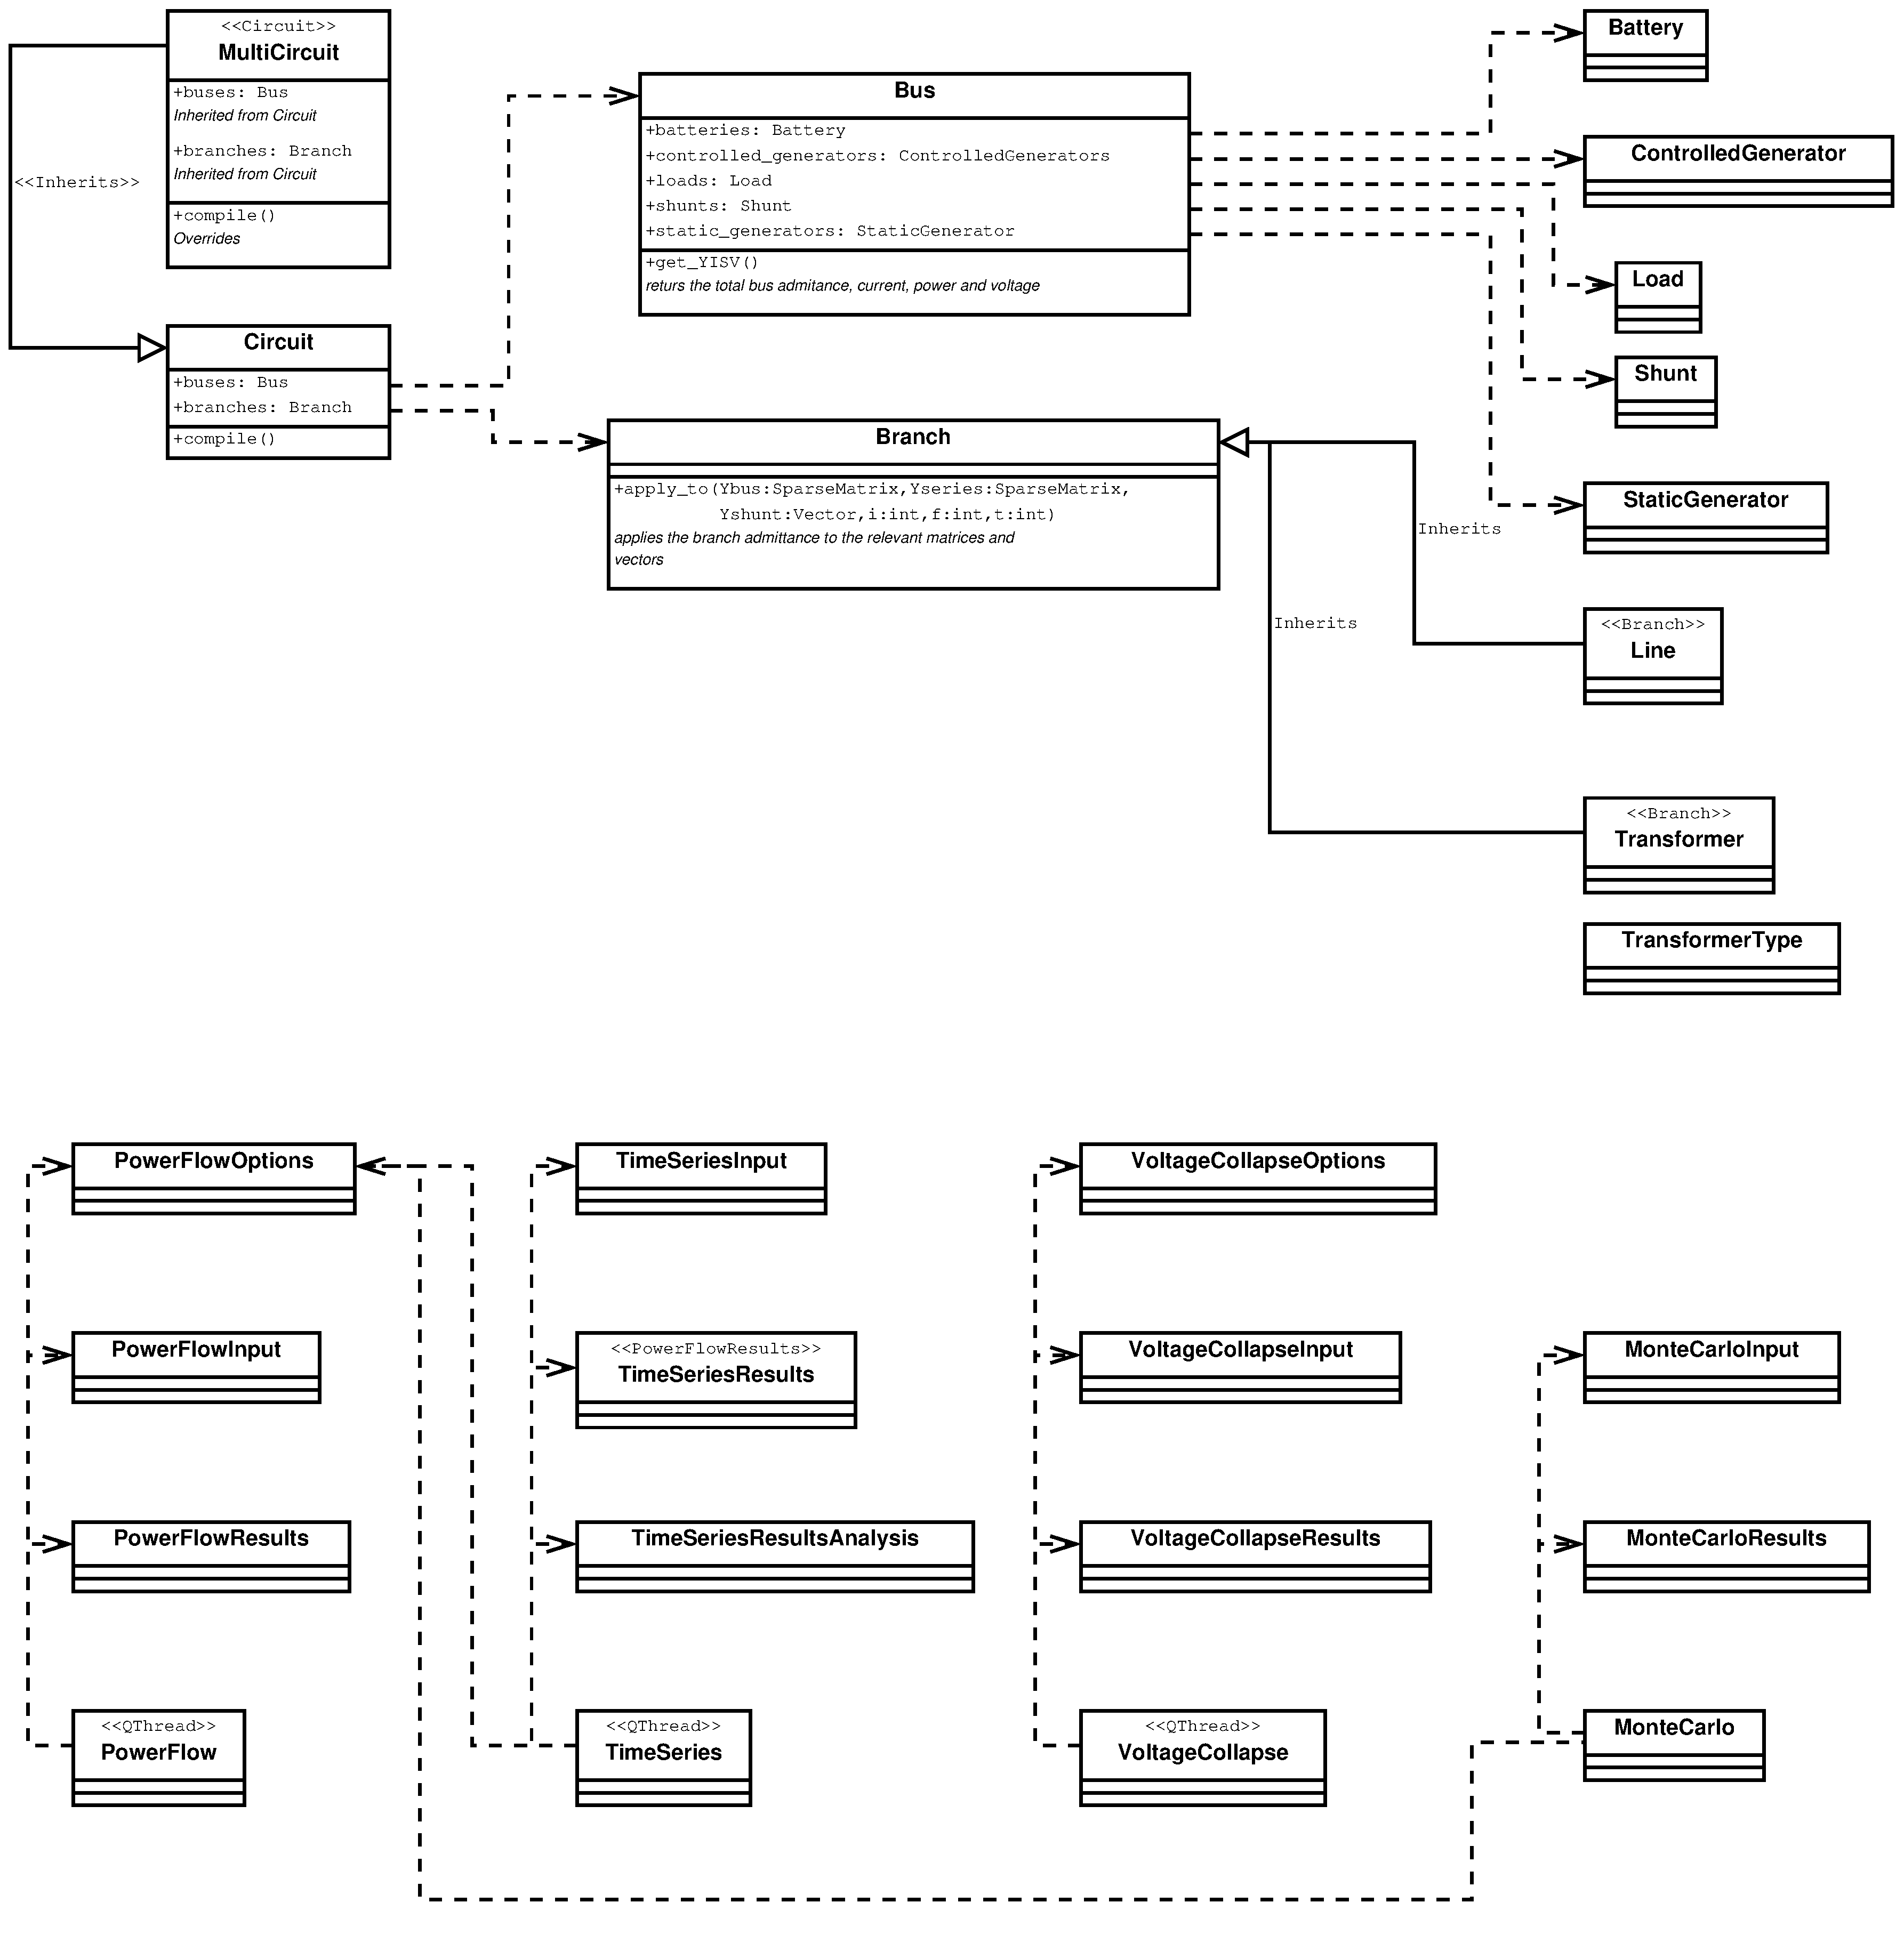
\includegraphics[width=1.0\linewidth]{ClassDiagram.eps}
	\caption{Simplified class diagram of GridCal's API}
	\label{fig:ClassDiagram}
\end{figure}

%----------------------------------------------------------------------------------------
%	CHAPTER 3
%----------------------------------------------------------------------------------------

\chapterimage{chapterhdr1.jpg} % Chapter heading image
\chapter{Models}



\section{Building the admittance matrices} \label{admitances_section}

This operation occurs in the \verb|Compile()| function of the \verb|Circuit| object. This function compiles many other magnitudes and among them, the following matrices:

\begin{itemize}
	\item \verb|Ybus|: Complete admittance matrix.
	
	It is a sparse matrix of size $n \times n$
	
	\item \verb|Yseries|: Admittance matrix of the series elements. It contains no value comming from shunt elements or the shunt parts of the branch model.
	
	It is a sparse matrix of size $n \times n$
	
	\item \verb|Yshunt|: Admittance vector of the shunt elements and the shunt parts of the branch model. 
	
	It is a vector of size $n$
	
	\item \verb|Yf|: Admittance matrix of the banches with their \textit{from} bus.
	
	It is a sparse matrix of size $m \times n$
	 
	\item \verb|Yt|: Admittance matrix of the banches with their \textit{to} bus.
	
	It is a sparse matrix of size $m \times n$\newline
\end{itemize}

Where $n$ is the number of buses and $m$ is the number of branches.

The relation between the admittance matrix and the series and shunt admittance matrices is the following:
\begin{equation}
Y_{bus} = Y_{series} + Y_{shunt}
\end{equation}

The algorithmic logic to build the matrices in pseudo code is the following:

\begin{verbatim}
n = number of buses in the circuit
m = number of branches in the circuit
For i=0 to n:
   bus_shunt_admittance, bus_current, bus_power, bus_voltage = buses[i].get_YISV()
   
   Yshunt[i] = bus_shunt_admittance
end

For i=0 to m:
   f = get_bus_inde(branches[i].bus_from)
   t = get_bus_inde(branches[i].bus_to)
   
   // the matrices are modified by the branch object itself
   branches[i].apply_to(Ybus,Yseries,Yshunt,Yf,Yt,i,f,t)
end
	
\end{verbatim}

\section{The universal branch model}\label{Universal_branch_model}

The following describes the model that is applied to each type of admittance matrix in the \verb|apply_to()| function inside the \verb|Branch| object seen before.

The model implemented to describe the behavior of the transformers and lines is the $\pi$ (pi) model.
\begin{figure}[h]
	\centering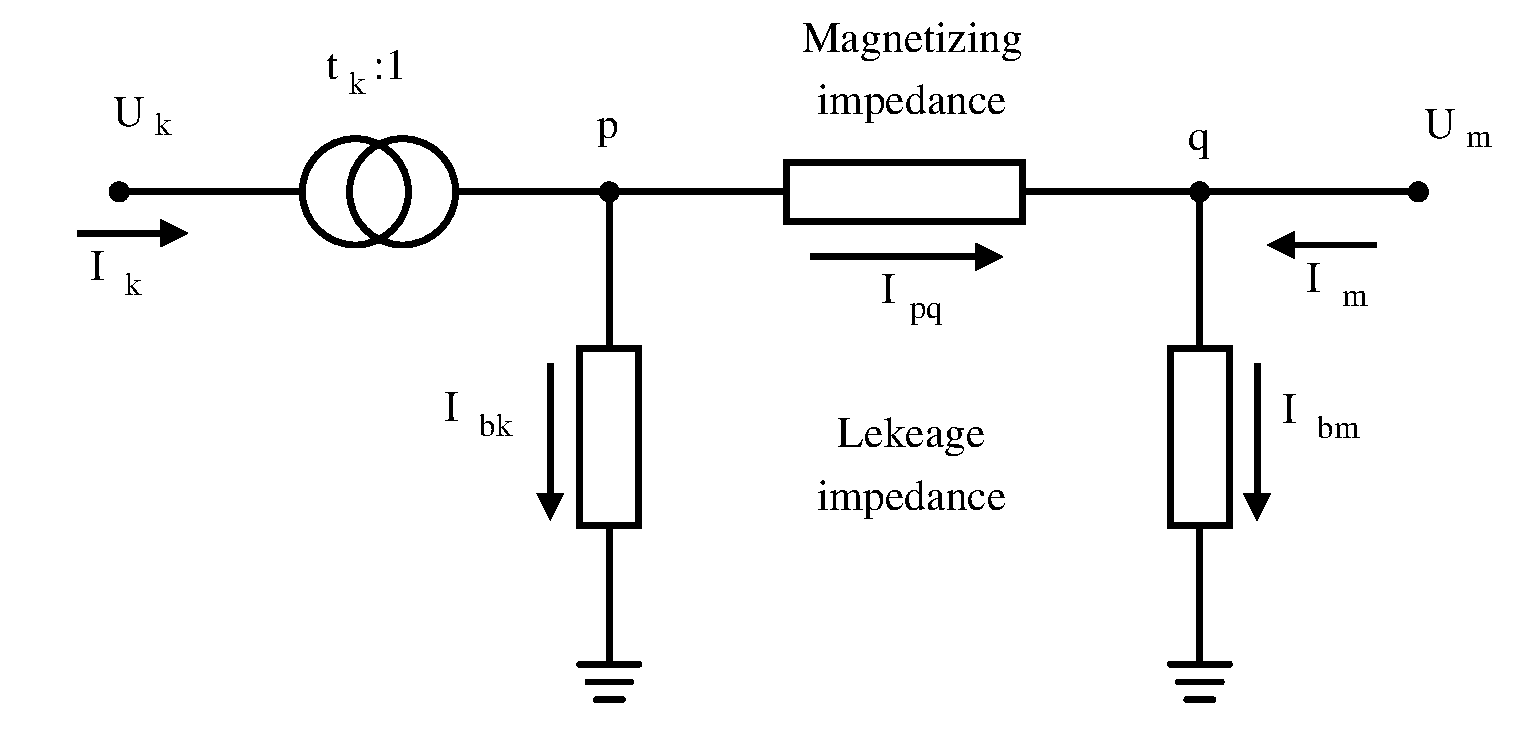
\includegraphics[width=0.8\linewidth]{pi-trafo.eps}
	\caption{$\pi$ model of a branch}
	\label{trafo pi model}
\end{figure}

To define the $\pi$ branch model we need to specify the following magnitudes:

\begin{itemize}
	\item $z_{series}$: Magnetizing impedance or simply series impedance. It is given in p.u.
	\item $y_{shunt}$: Leakage impedance or simply shunt impedance. It is given in p.u.
	\item $tap\_module$: Module of the tap changer. It is a magnitude around 1.
	\item $tap\_angle$: Angle of the tap changer. Angle in radians.\newline
\end{itemize}


%tap = self.tap_module * exp(-1j * self.angle)

In order to apply the effect of a branch to the admittance matrices, first we compute the complex tap value.
$$tap = tap\_module \cdot e^{-j \cdot tap\_angle}$$  

Then we compose the equivalent series and shunt admittance values of the branch. Both values are complex.
%Ys = 1 / self.z_series
$$Y_s = \frac{1}{z_{series}}$$
%Ysh = self.y_shunt / 2
$$Y_{sh} = \frac{y_{shunt}}{2}$$

\begin{itemize}
	\item $z_{series}$: Series impedance of the branch composed by the line resistance and its inductance. $z_{series}=r + jl$
	
	\item $y_{shunt}$: Shunt admittance of the line composed by the conductance and the susceptance. $y_{shunt}=c+jb$\newline
\end{itemize}



The general branch model is represented by a $2 \times 2$ matrix.
$
Y_{branch}=\left( \begin{array}{ccc}
Y_{ff} & Y_{ft} \\
Y_{tf} & Y_{tt} \end{array} \right)
$

In this matrix, the elements are the following:

%Yff = Ytt / (tap * conj(tap))
%Yft = - Ys / conj(tap)
%Ytf = - Ys / tap
%Ytt = Ys + Ysh

$$Y_{ff} = \frac{Y_s + Y_{sh}}{tap \cdot conj(tap)}  $$
$$Y_{ft} = - Y_s / conj(tap)$$
$$Y_{tf} = - Y_s / tap$$
$$Y_{tt} = Y_s + Y_{sh}$$

\subsubsection{Ybus}

The branch admittance values are applied to the complete admittance matrix as follows:

%Ybus[f, f] += Yff
%Ybus[f, t] += Yft
%Ybus[t, f] += Ytf
%Ybus[t, t] += Ytt
$${Y_{bus}}_{f, f} = {Y_{bus}}_{f, f}  + Y_{ff}$$
$${Y_{bus}}_{f, t} = {Y_{bus}}_{f, t} + Y_{ft}$$
$${Y_{bus}}_{t, f} = {Y_{bus}}_{t, f} + Y_{tf}$$
$${Y_{bus}}_{t, t} = {Y_{bus}}_{t, t} + Y_{tt}$$


These formulas assume that there might be something already in $Y_{bus}$, therefore the right way to modify these values is to add the own branch values.


\subsection{Yshunt}
%Yff_sh = Ysh
%Ytt_sh = Yff_sh / (tap * conj(tap))
%Yshunt[f] += Yff_sh
%Yshunt[t] += Ytt_sh
$${Y_{shunt}}_f = {Y_{shunt}}_f  + Y_{sh}$$
$${Y_{shunt}}_t = {Y_{shunt}}_t  + \frac{Y_{sh}}{tap \cdot conj(tap)}$$

\subsection{Yseries}
%Yseries[f, f] += Ys / (tap * conj(tap))
%Yseries[f, t] += Yft
%Yseries[t, f] += Ytf
%Yseries[t, t] += Ys

$${Y_{series}}_{f, f} = {Y_{series}}_{f, f}  + \frac{Y_{s}}{tap \cdot conj(tap)}$$
$${Y_{series}}_{f, t} = {Y_{series}}_{f, t} + Y_{ft}$$
$${Y_{series}}_{t, f} = {Y_{series}}_{t, f} + Y_{tf}$$
$${Y_{series}}_{t, t} = {Y_{series}}_{t, t} + Y_{s}$$

\subsection{Yf and Yt}
%# Yf = csr_matrix((r_[Yff, Yft], (i, r_[f, t])), (nl, nb))
%# Yt = csr_matrix((r_[Ytf, Ytt], (i, r_[f, t])), (nl, nb))

%Yf[i, f] += Yff  # Ybus[f, f]
%Yf[i, t] += Yft  # Ybus[f, t]
$${Y_f}_{i, f} = {Y_f}_{i, f} + Y_{ff}$$
$${Y_f}_{i, t} = {Y_f}_{i, t} + Y_{ft}$$

%Yt[i, f] += Ytf  # Ybus[t, f]
%Yt[i, t] += Ytt  # Ybus[t, t]
$${Y_t}_{i, f} = {Y_t}_{i, f} + Y_{tf}$$
$${Y_t}_{i, t} = {Y_t}_{i, t} + Y_{tt}$$

Here $i$ is the index of the branch in the circuit and $f$, $t$ are the corresponding bus indices.


\section{The transformer definition from the short circuit test values}
\label{Transformer_definition}

The transformers are modeled as $\pi$ branches too. In order to get the series impedance and shunt admittance of the transformer to match the branch model, it is advised to transform the specification sheet values of the device into the desired values. The values to take from the specs sheet are: \newline
\begin{itemize}
	\item $S_n$: Nominal power in MVA.
	\item $U_{hv}$: Voltage at the high-voltage side in kV.
	\item $U_{lv}$: Voltage at the low-voltage side in kV.
	\item $U_{sc}$: Short circuit voltage in \%.
	\item $P_{cu}$: Copper losses in kW.
	\item $I_0$: No load current in \%.
	\item $GX_{hv1}$: Reactance contribution to the HV side. Value from 0 to 1.
	\item $GR_{hv1}$: Resistance contribution to the HV side Value from 0 to 1.\newline
\end{itemize}

Then, the series and shunt impedances are computed as follows:

Nominal impedance HV (Ohm): $Zn_{hv} = U_{hv}^2 / S_n$ \newline


Nominal impedance LV (Ohm): $Zn_{lv} = U_{lv}^2 / S_n$ \newline


Short circuit impedance (p.u.): $z_{sc} = U_{sc} / 100$\newline

Short circuit resistance (p.u.): $r_{sc} = \frac{P_{cu} / 1000}{S_n}$\newline

Short circuit reactance (p.u.): $x_{sc} = \sqrt{z_{sc}^2 - r_{sc} ^2}$\newline


HV resistance (p.u.): $r_{cu,hv} = r_{sc} \cdot GR_{hv1}$\newline


LV resistance (p.u.): $r_{cu,lv} = r_{sc} \cdot (1 - GR_{hv1})$\newline


HV shunt reactance (p.u.): $xs_{hv} = x_{sc} \cdot GX_{hv1}$\newline


LV shunt reactance (p.u.): $xs_{lv} = x_{sc} \cdot (1 - GX_{hv1})$\newline

Shunt resistance (p.u.): $r_{fe} = \frac{Sn}{P_{fe} / 1000}$\newline


Magnetization impedance (p.u.): $z_m = \frac{1}{I_0 / 100}$\newline

Magnetization reactance (p.u.): $x_m = \frac{1}{\sqrt{\frac{1}{z_m^2} - \frac{1}{r_{fe}^2}}}$ \newline

If the content of the square root is negative, set the magnetization impedance to zero.\\


The final complex calculated parameters in per unit are:

Magnetizing impedance (or series impedance): $z_{series} = Z_m = r_{fe} +j \cdot x_m$

Leakage impedance (or shunt impedance): $Z_l = r_{sc} + j \cdot x_{sc}$

Shunt admittance: $y_{shunt} = 1 / Z_l$


\subsection{Inverse definition of short-circuit values from the $\Pi$ model}

In GridCal I found the need to find the short circuit values ($P_{cu}$, $V_{sc}$, $r_{fe}$, $I0$) from the branch values ($R$, $X$, $G$, $B$). Hence the following formulas:

%zsc = sqrt(R * R + 1 / (X * X))
%Vsc = 100.0 * zsc
%Pcu = R * Sn * 1000.0
%
%if abs(G) > 0.0 and abs(B) > 0.0:
%zl = 1.0 / complex(G, B)
%rfe = zl.real
%xm = zl.imag
%
%Pfe = 1000.0 * Sn / rfe
%
%k = 1 / (rfe * rfe) + 1 / (xm * xm)
%I0 = 100.0 * sqrt(k)
%else:
%Pfe = 0
%I0 = 0

\begin{equation}
z_{sc} = \sqrt{R^2 + 1 / X^2}
\end{equation}


\begin{equation}
V_{sc} = 100 \cdot z_{sc}
\end{equation}

\begin{equation}
P_{cu} = R \cdot S_n \cdot 1000
\end{equation}

\begin{equation}
zl = 1 / (G + j B)
\end{equation}

\begin{equation}
r_{fe} = zl.real
\end{equation}

\begin{equation}
xm = zl.imag
\end{equation}

\begin{equation}
I0 = 100 \cdot \sqrt{1 / r_{fe}^2 + 1 / xm^2}
\end{equation}


%----------------------------------------------------------------------------------------
%	CHAPTER 4
%----------------------------------------------------------------------------------------

\chapterimage{chapterhdr1.jpg} % Chapter heading image

\chapter{Power flow}

\section{Newton-Raphson-Iwamoto}

The Newton-Raphson method is the standard power flow method tough at schools. GridCal implements a slight but important modification of this method that turns it into a more robust, industry-standard algorithm. The Newton Raphson method is the first order Taylor approximation of the power flow equation. The method implemented in GridCal is the second order approximation, let's see how.

The expression to update the voltage solution in the Newton-Raphson algorithm is the following:
\begin{equation}
\textbf{V}_{t+1} = \textbf{V}_t + \textbf{J}^{-1}(\textbf{S}_0 - \textbf{S}_{calc})
\end{equation}

Where:
\begin{itemize}
	\item $\textbf{V}_t$: Voltage vector at the iteration $t$  (current voltage) 
	\item $\textbf{V}_{t+1}$: Voltage vector at the iteration $t+1$  (new voltage)
	\item $\textbf{J}$: Jacobian matrix.
	\item $\textbf{S}_0$: Specified power vector.
	\item $\textbf{S}_{calc}$: Calculated power vector using $\textbf{V}_t$.\newline
\end{itemize}

In matrix form we get:

%J11 = dS_dVa[array([pvpq]).T, pvpq].real
%J12 = dS_dVm[array([pvpq]).T, pq].real
%J21 = dS_dVa[array([pq]).T, pvpq].imag
%J22 = dS_dVm[array([pq]).T, pq].imag

\begin{equation}
\begin{bmatrix}
J_{11} & J_{12} \\
J_{21} & J_{22} \\
\end{bmatrix}
\times
\begin{bmatrix}
\Delta\theta\\
\Delta|V|\\
\end{bmatrix}
=
\begin{bmatrix}
\Delta P\\
\Delta Q\\
\end{bmatrix}
\end{equation}



The formulation implemented in GridCal includes the optimal acceleration parameter $\mu$:

\begin{equation}
\textbf{V}_{t+1} = \textbf{V}_t + \mu \textbf{J}^{-1}(\textbf{S}_0 - \textbf{S}_{calc})
\end{equation}

Here $\mu$ is the Iwamoto optimal step size parameter. In 1982 S.Iwamoto and Y.Tamura present a method \cite{iwamoto1981load} where the Jacobian matrix $J$ is only computed at the beginning, and the iteration control parameter $\mu$ is computed on every iteration. In GridCal I compute $J$ and $\mu$ on every iteration getting a more robust method on the expense of a greater computational effort.

To compute the parameter $\mu$ we must do the following:

\begin{theorem}[Computation of $\mu$]
$$\textbf{J'} = Jacobian(\textbf{Y}, \textbf{dV})$$
$$\textbf{dx} = \textbf{J}^{-1}(\textbf{S}_0 - \textbf{S}_{calc})$$
$$\textbf{a} = \textbf{S}_0 - \textbf{S}_{calc}$$
$$\textbf{b} = \textbf{J} \times \textbf{dx}$$
$$\textbf{c} = \frac{1}{2} \textbf{dx} \cdot (\textbf{J'} \times \textbf{dx})$$

$$g_0 = -\textbf{a} \cdot \textbf{b}$$
$$g_1 = \textbf{b} \cdot \textbf{b} + 2  \textbf{a} \cdot \textbf{c}$$
$$g_2 = -3  \textbf{b} \cdot \textbf{c}$$
$$g_3 = 2  \textbf{c} \cdot \textbf{c}$$

$$G(x) = g_0 + g_1x + g_2x^2 + g_3x^3$$

$$\mu = solve(G(x), x_0=1)$$
\end{theorem}


There will be three solutions to the polynomial $G(x)$. Only the last solution will be real, and therefore it is the only valid value for $\mu$.
The polynomial can be solved numerically using $1$ as the seed.

The matrix $\textbf{J'}$ is the Jacobian matrix computed using the voltage derivative numerically computed as the voltage increment $\textbf{dV}= \textbf{V}_{t} - \textbf{V}_{t-1}$ (voltage difference between the current and the previous iteration).  

\newpage
\subsection{Jacobian}

The Jacobian matrix is the derivative of the power flow equation for a given voltage set of values.

\begin{equation}
J =
\begin{bmatrix}
J_{11} & J_{12} \\
J_{21} & J_{22} \\
\end{bmatrix}
\end{equation}

Where:

\begin{itemize}
	\item $J11 = Re(\frac{\partial S}{\partial \theta}[pvpq, pvpq])$  
	\item $J12 = Re(\frac{\partial S}{\partial |V|}[pvpq, pq])$
	\item $J21 = Im(\frac{\partial S}{\partial \theta}[pq, pvpq])$
	\item $J22 = Im(\frac{\partial S}{\partial |V|}[pq pq])$\newline
\end{itemize}

Here we introduced two complex-valued derivatives:\newline

\begin{itemize}
	\item $\frac{\partial S}{\partial \theta} = V_{diag} \cdot (Y_{bus} \times V_{diag,norm})^* + I_{diag}^* \cdot V_{diag,norm}$ 
	\item $\frac{\partial S}{\partial |V|} =  1j \cdot V_{diag} \cdot (I_{diag} - Y_{bus} \times V_{diag})^*$\newline
\end{itemize}

Where:

\begin{itemize}
	\item $V_{diag}$: Diagonal matrix formed by a voltage solution.
	\item $V_{diag,norm}$: Diagonal matrix formed by a voltage solution, where every voltage is divided by its module.
	\item $I_{diag}$: Diagonal matrix formed by the current injections.
	\item $Y_{bus}$: And of course, this is the circuit full admittance matrix. \newline
\end{itemize}

This Jacobian form can be used for other methods.

\section{Levenberg-Marquardt}

The Levenberg-Marquardt iterative method is often used to solve non-linear least squares problems. in those problems one reduces the calculated error by iteratively solving a system of equations that provides the increment to add to the solution in order to decrease the solution error. So conceptually it applies to the power flow problem.

%\begin{theorem}[Levenberg-Marquardt algorithm]
%	$$\textbf{J} = Jacobian(\textbf{Y}, \textbf{V})$$
%\end{theorem}
Set the initial values:
\begin{itemize}
	\item $\nu=2$
	\item $f_{prev} = 10^9$
	\item $ComputeH = true$
\end{itemize}

In every iteration:
\begin{itemize}
	\item Compute the jacobian matrix if $ComputeH$ is $true$: 
	$$\textbf{H} = Jacobian(\textbf{Y}, \textbf{V})$$
	\item Compute the mismatch in the same order as the jacobian:
	$$\textbf{S}_{calc} = \textbf{V} (\textbf{Y} \cdot \textbf{V} - \textbf{I})^*$$
	$$\textbf{m} = \textbf{S}_{calc} - \textbf{S}$$
	$$\textbf{dz} = [ Re(\textbf{m}_{pv}), Re(\textbf{m}_{pq}), Im(\textbf{m}_{pq})]$$
	\item Compute the auxiliary jacobian transformations:
	$$\textbf{H}_1 = \textbf{H}^\top$$
	$$\textbf{H}_2 = \textbf{H}_1 \cdot \textbf{H}$$
	\item Compute the first value of $\lambda$ (only in the first iteration): 
	$$\lambda = 10^{-3} Max(Diag(\textbf{H}_2))$$
	\item Compute the system Matrix:
	$$\textbf{A} = \textbf{H}_2 + \lambda \cdot Identity $$
	\item Compute the linear system right hand side:
	$$\textbf{rhs} = \textbf{H}_1 \cdot \textbf{dz} $$
	\item Solve the system increment:
	$$\textbf{dx} = Solve(\textbf{A}, \textbf{rhs})$$
	\item Compute the objective function:
	$$f = 0.5 \cdot \textbf{dz} \cdot \textbf{dz}^\top  $$
	\item Compute the decision function:
	$$\rho = \frac{f_{prev}-f}{0.5 \cdot \textbf{dx}^\top \cdot (\lambda \textbf{dx} + \textbf{rhs})} $$
	\item Update values: \newline
	If $\rho > 0$
	\begin{itemize}
		\item $ComputeH = true$
		\item $\lambda = \lambda \cdot max(1/3, 1- (2 \cdot \rho -1)^3)$
		\item $\nu = 2$
		\item Update the voltage solution using $\textbf{dx}$.
	\end{itemize}
	Else
	\begin{itemize}
		\item $ComputeH = false$
		\item $\lambda = \lambda \cdot \nu$
		\item $\nu = \nu \cdot 2$
	\end{itemize}
	\item Compute the convergence: 
	$$converged = ||dx, \infty|| < tolerance $$
	\item $f_{prev} = f$\newline
\end{itemize}

As you can see it takes more steps than Newton-Raphson. It is a slower method, but it works better for ill-conditioned and large grids.


\newpage
\section{DC approximation}

The so called direct current power flow (or just DC power flow) is a convenient oversimplification of the power flow procedure.

It assumes that in any branch the reactive part of the impedance is much larger than the resistive part, hence the resistive part is neglected, and that all the voltages modules are the nominal per unit values. This is, $|v|=1$ for load nodes and $|v|=v_{set}$ for the generator nodes, where $v_{set}$ is the generator set point value.

In order to compute the DC approximation we must perform a transformation. The slack nodes are removed from the grid, and their influence is maintained by introducing equivalent currents in all the nodes. The equivalent admittance matrix ($\textbf{Y}_{red}$) is obtained by removing the rows and columns corresponding to the slack nodes. Likewise the removed elements conform the ($\textbf{Y}_{slack}$) matrix.

\begin{figure}[h!]
	\centering
	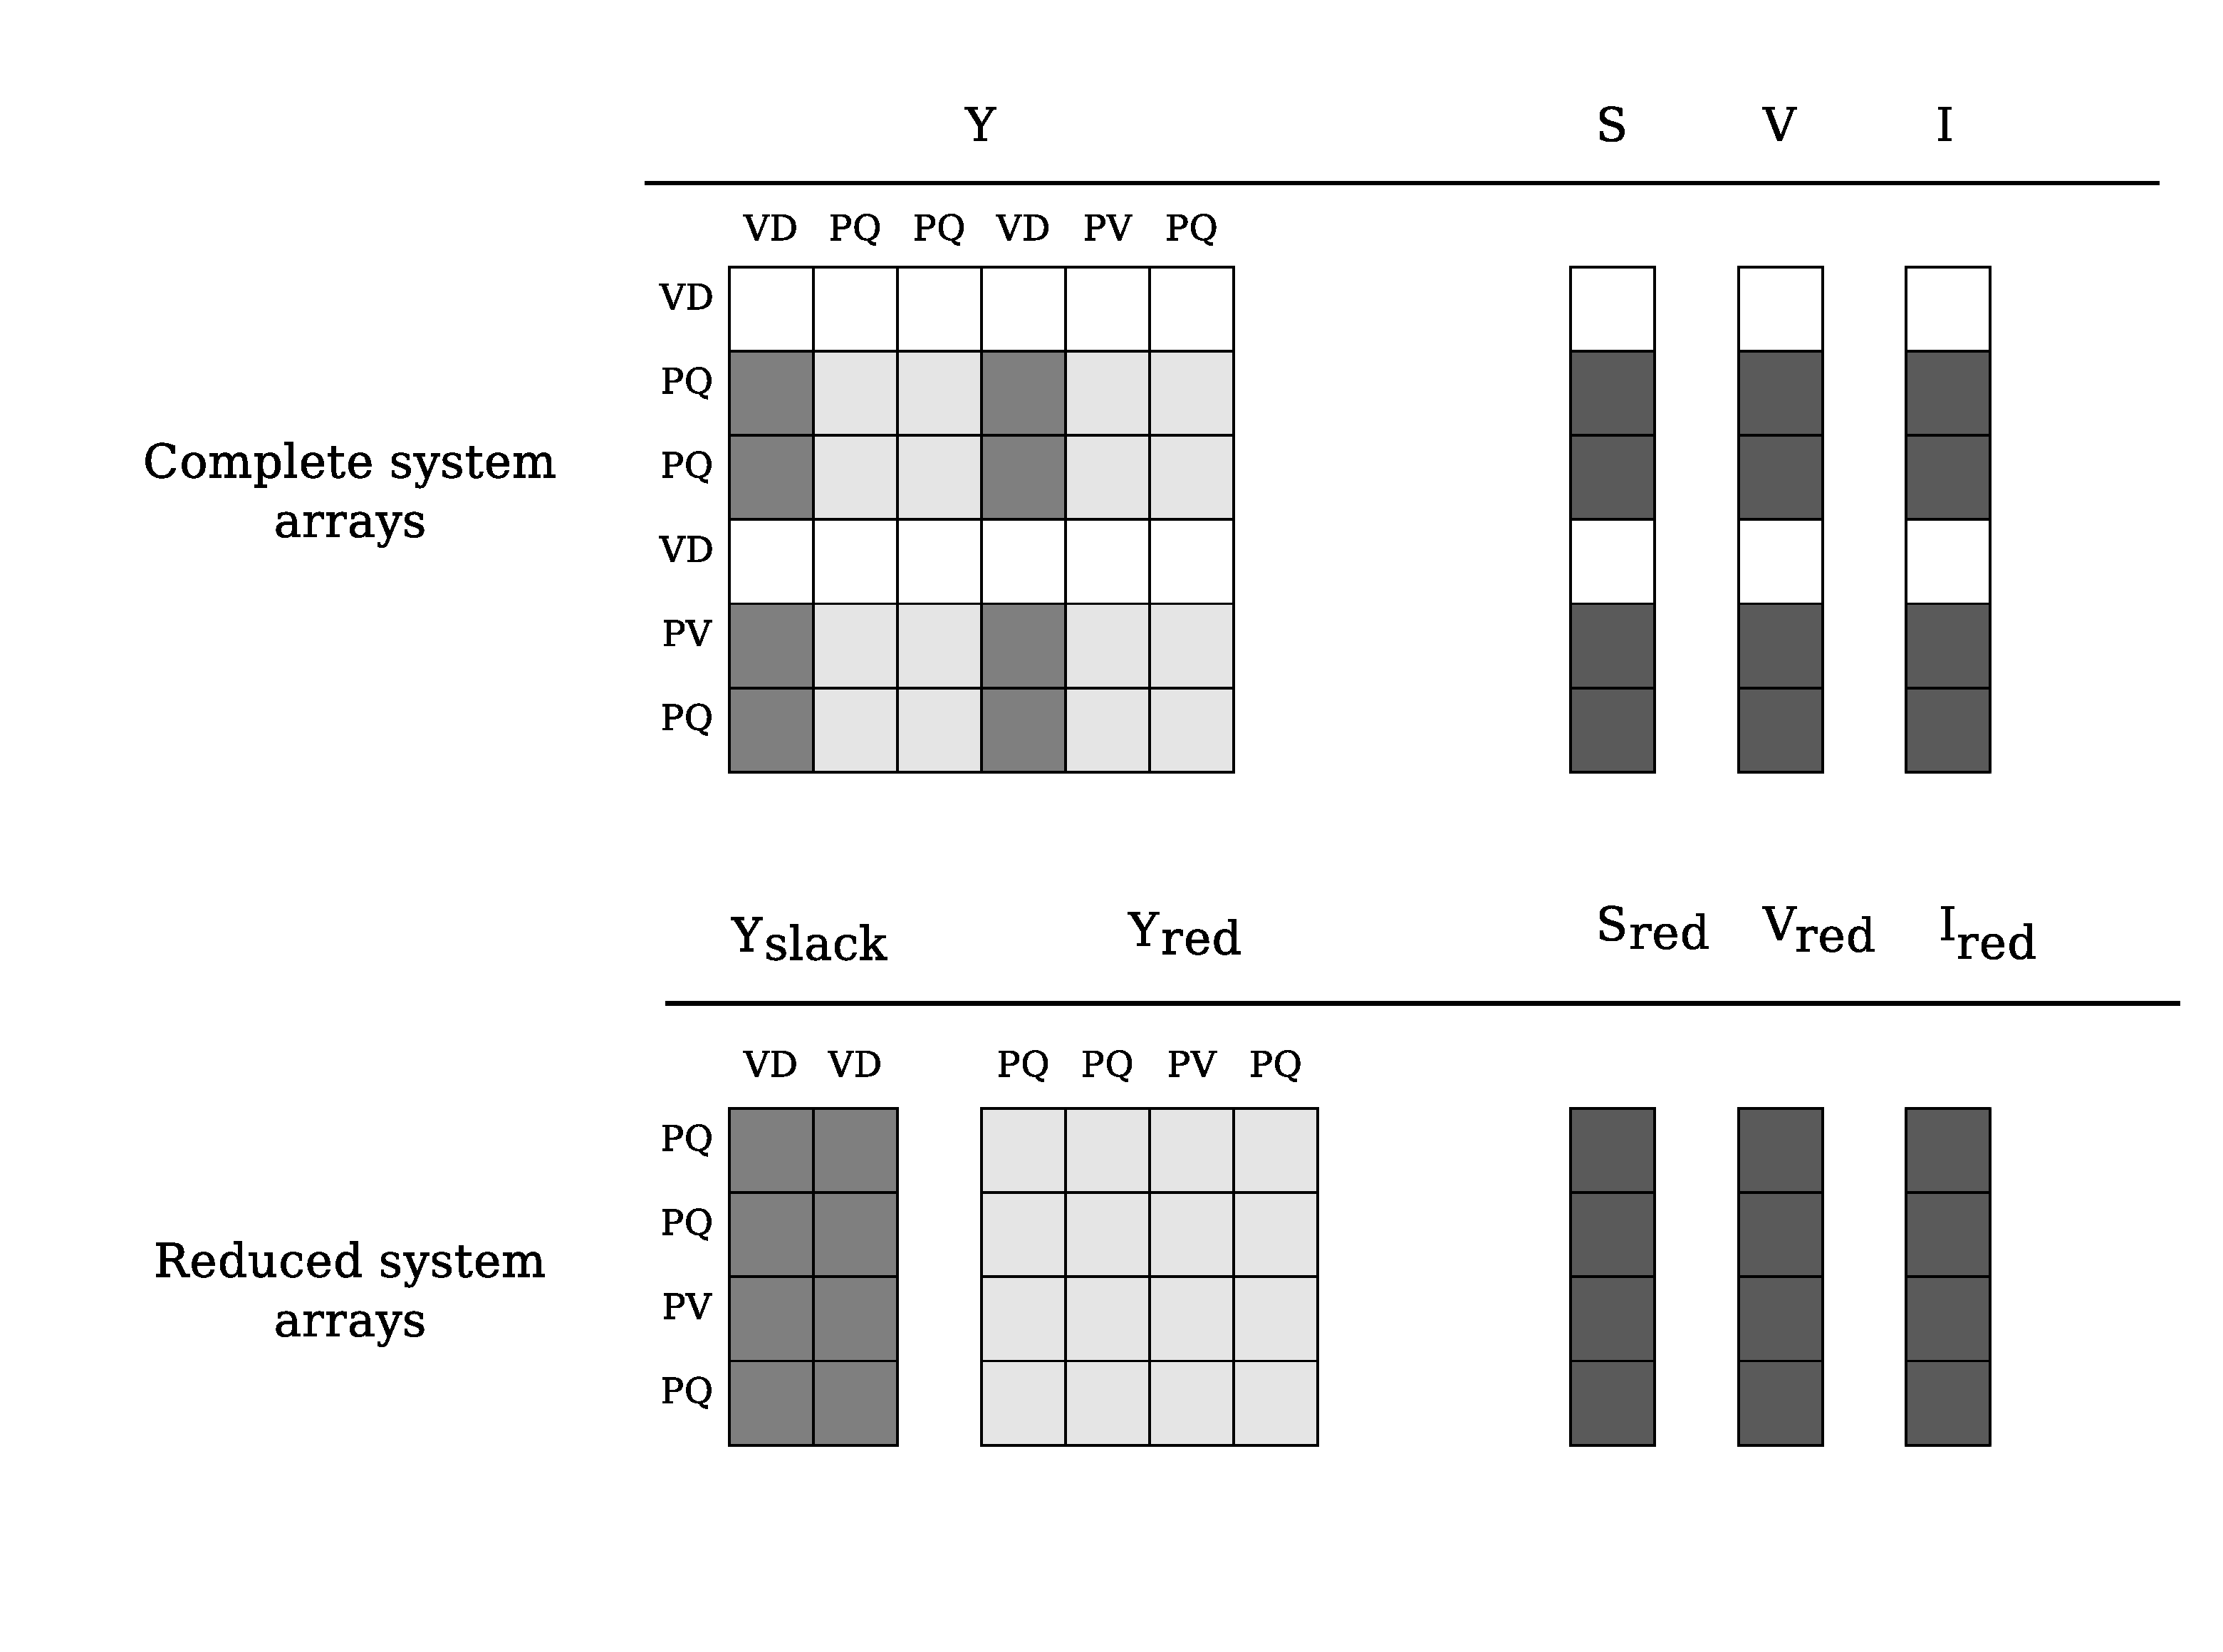
\includegraphics[width=0.55\linewidth]{Matrix_reduction.eps}
	\caption{Matrix reduction (VD: Slack, PV: Voltage controlled, PQ: Power controlled)}
	\label{fig:Matrix_reduction}
\end{figure}

%# Decompose the voltage in angle and magnitude
%Va_ref = angle(V0[ref])  # we only need the angles at the slack nodes
%Vm = npabs(V0)
%
%# initialize result vector
%Va = empty(len(V0))
%
%# reconvert the pqpv vector to a matrix so that we can call numpy directly with it
%pvpq_ = matrix(pvpq)
%
%# Compile the reduced imaginary impedance matrix
%Bpqpv = Ybus.imag[pvpq_.T, pvpq_]
%Bref = Ybus.imag[pvpq_.T, ref]
%
%# compose the reduced power injections
%# Since we have removed the slack nodes, we must account their influence as injections Bref * Va_ref
%Pinj = Sbus[pvpq].real - Bref * Va_ref + Ibus[pvpq].real
%
%# update angles for non-reference buses
%Va[pvpq] = spsolve(Bpqpv, Pinj)
%Va[ref] = Va_ref
%
%# re assemble the voltage
%V = Vm * exp(1j * Va)
%
%# compute the calculated power injection and the error of the voltage solution
%Scalc = V * conj(Ybus * V - Ibus)
%
%# compute the power mismatch between the specified power Sbus and the calculated power Scalc
%mis = Scalc - Sbus  # complex power mismatch
%F = r_[mis[pv].real, mis[pq].real, mis[pq].imag]  # concatenate again
%
%# check for convergence
%normF = linalg.norm(F, Inf)

\begin{equation}
\textbf{P} = real(\textbf{S}_{red}) + (- imag(\textbf{Y}_{slack}) \cdot angle(\textbf{V}_{slack}) + real(\textbf{I}_{red})) \cdot |\textbf{V}_{red}|
\label{dc_power_injections}
\end{equation}

The equation \ref{dc_power_injections} computes the DC power injections as the sum of the different factors mentioned:

\begin{enumerate}
	\item $real(\textbf{S}_{red})$: Real part of the reduced power injections.
	\item $imag(\textbf{Y}_{slack}) \cdot angle(\textbf{V}_{slack}) \cdot |v_{red}|$: Currents that appear by removing the slack nodes while keeping their influence, multiplied by the voltage module to obtain power.
	\item $real(\textbf{I}_{red}) \cdot |v_{red}|$: Real part of the grid reduced current injections, multiplied by the voltage module to obtain power.
\end{enumerate}

Once the power injections are computed, the new voltage angles are obtained by:

\begin{equation}
\textbf{V}_{angles} = imag(\textbf{Y}_{red})^{-1} \times \textbf{P}
\end{equation}

The new voltage is then:
\begin{equation}
\textbf{V}_{red} = |\textbf{V}_{red}| \cdot e^{1j \cdot  \textbf{V}_{angles}}
\end{equation}

This solution does usually produces a large power mismatch. That is to be expected because the method is an oversimplification with no iterative convergence criteria, just a straight forward set of operations.

\newpage
\section{Linear AC power flow}

Following the formulation presented in \cite{rossoni2016linearized}, we obtain a way to solve circuits in one shot (without iterations) and quite positive results for a linear approximation.

\begin{equation}
\begin{bmatrix}
A_{11} & A_{12} \\
A_{21} & A_{22} \\
\end{bmatrix}
\times
\begin{bmatrix}
\theta\\
|V|\\
\end{bmatrix}
=
\begin{bmatrix}
Rhs_1\\
Rhs_2\\
\end{bmatrix}
\end{equation}

Where:
\begin{itemize}
	\item $A_{11} = -Im(Y_{series}[pqpv, pqpv])$
	\item $A_{12} = Re(Y_{bus}[pqpv, pq])$
	\item $A_{21} = -Im(Y_{series}[pq, pqpv])$
	\item $A_{22} = -Re(Y_{bus}[pq, pq])$
	\item $Rhs_1 = P[pqpv]$
	\item $Rhs_2 = Q[pq]$\newline
\end{itemize}

Here, $Y_{bus}$ is the normal circuit admittance matrix and $Y_{series}$ is the admittance matrix formed with only series elements of the $\pi$ model, this is neglecting all the shunt admittances.

Solving the vector $[\theta, |V|]$ we get $\theta$ for the pq and pv nodes and $|V|$ for the pq nodes.\newline

For equivalence with the paper:\newline

\begin{itemize}
	\item $-B' = -Im(Y_{series}[pqpv, pqpv])$
	\item $G = Re(Y_{bus}[pqpv, pq])$
	\item $-G' = -Im(Y_{series}[pq, pqpv])$
	\item $-B = -Re(Y_{bus}[pq, pq])$\newline
\end{itemize}

\newpage
\section{Holomorphic Embedding}

First introduced by Antonio Trias in 2012 \cite{TriasHELM}, promises to be a non-divergent power flow method. Trias originally developed a version with no voltage controlled nodes (PV), in which the convergence properties are excellent (With this software try to solve any grid without PV nodes to check this affirmation). 

The version programmed in the file \verb|HELM.py| has been adapted from the master thesis of Muthu Kumar Subramanian at the Arizona State University (ASU) \cite{subramanian2014application}. This version includes a formulation of the voltage controlled nodes. My experience indicates that the introduction of the PV control deteriorates the convergence properties of the holomorphic embedding method. However, in many cases, it is the best approximation to a solution. especially when Newton-Raphson does not provide one.

The file \verb|HELM.py| contains a vectorized version of the algorithm. This means that the execution in python is much faster than a previous version that uses loops.

\subsection{Concepts}

All the power flow algorithms until the HELM method was introduced were iterative and recursive. The helm method is iterative but not recursive. A simple way to think of this is that traditional power flow methods are exploratory, while the HELM method is a planned journey. In theory the HELM method is superior, but in practice the numerical degeneration makes it less ideal.

The fundamental idea of the recursive algorithms is that given a voltage initial point (1 p.u. at every node, usually) the algorithm explores the surroundings of the initial point until a suitable voltage solution is reached or no solution at all is found because the initial point is supposed to be "far" from the solution.

On the HELM methods, we form a "curve" that departures from a known mathematically exact solution that is obtained from solving the grid with no power injections. This is possible because with no power injections, the grid equations become linear and straight forward to solve. The arriving point of the "curve" is the solution that we want to achieve. That "curve" is best approximated by a Padè approximation. To compute the Padè approximation we need to compute the coefficients of the unknown variables, in our case the voltages (and possibly the reactive powers at the PV nodes).

The HELM formulation consists in the derivation of formulas that enable the calculation of the coefficients of the series that describes the "curve" from the mathematically know solution to the unknown solution. Once the coefficients are obtained, the Padè approximation computes the voltage solution at the "end of the curve", providing the desired voltage solution. The more coefficients we compute the more exact the solution is (this is true until the numerical precision limit is reached).\newline 


All this sounds very strange, but it works ;)\newline 


If you want to get familiar with this concept, you should read about the homotopy concept. In practice the continuation power flow does the same as the HELM algorithm, it takes a known solution and changes the loading factors until a solution for another state is reached.

\subsection{Fundamentals} \label{helm_fundamentals}

The fundamental equation that defines the power flow problem is:
\begin{equation}
\textbf{S} = \textbf{V} \times (\textbf{Y} \times \textbf{V})^*
\end{equation}

Most usefully represented like this:


\begin{equation}
{\textbf{Y} \times \textbf{V}} = \left(\frac{\textbf{S}}{\textbf{V}}\right)^* 
\label{base_eq}
\end{equation}


The holomorphic embedding is to insert a "travelling" parameter $\alpha$, such that for $\alpha=0$ we have an mathematically exact solution of the problem (but not the solution we're looking for...), and for $\alpha=1$ we have the solution we're looking for. The other thing to do is to represent the variables to be computed as McLaurin series. Let's go step by step.\newline

For $\alpha=0$ we say that $S=0$, in this way the equation \ref{base_eq} becomes linear, and its solution is mathematically exact. But for that to be useful in our case we need to split the admittance matrix $Y$ into $Y_{series}$ and $Y_{shunt}$. $Y_{shunt}$ is a diagonal matrix, so it can be expressed as a vector instead (no need for matrix-vector product).

\begin{equation}
\textbf{Y}_{series} \times \textbf{V} = \left(\frac{\textbf{S}}{\textbf{V}}\right)^* - \textbf{Y}_{shunt} \textbf{V}
\label{base_eq_alpha_0}
\end{equation}

This is what will allow us to find the zero "state" in the holomorphic series calculation. For $\alpha=1$ we say that $S=S$, so we don't know the voltage solution, however we can determine a path to get there:

\begin{equation}
{\textbf{Y }\times \textbf{V}( \alpha )} = \left(\frac{ \alpha\textbf{S}}{\textbf{V}( \alpha )}\right)^* - \alpha \textbf{Y}_{shunt} \times \textbf{V}( \alpha ) = \frac{ \alpha\textbf{S}^*}{\textbf{V}( \alpha )^*} - \alpha \textbf{Y}_{shunt} \textbf{V}( \alpha )
\label{base_eq_embedded}
\end{equation}

Wait, what?? did you just made this stuff up??, well so far my reasoning is:
\begin{itemize}
	\item The voltage $\textbf{V}$ is what I have to convert into a series, and the series depend of $\alpha$, so it makes sense to say that $\textbf{V}$, as it is dependent of $\alpha$, becomes $\textbf{V}(\alpha)$.
	
	\item Regarding the $\alpha$ that multiplies $\textbf{S}$, the amount of power ($\alpha \textbf{S}$) is what I vary during the \textit{travel} from $\alpha=0$ to $\alpha=1$, so that is why $\textbf{S}$ has to be accompanied by the \textit{traveling} parameter $\alpha.$
	
	\item In my opinion the $\alpha$ $\textbf{Y}_{shunt}$ is to provoke the first voltage coefficients to be one.  $\textbf{Y}_{series} \times \textbf{V}[0] = 0$, makes $V[0]=1$. This is essential for later steps (is a condition to be able to use Padè). \newline
\end{itemize}

The series are expressed as McLaurin equations:

\begin{equation}
V(\alpha) = \sum_{n}^{\infty} V_n \alpha ^n
\label{eq:McLaurinV}
\end{equation}

\begin{theorem}[Holomorphicity check]

	There's still something to do. The magnitude $\left(\textbf{V}( \alpha )\right)^*$ has to be converted into $\left(\textbf{V}( \alpha^* )\right)^*$. This is done in order to make the function be holomorphic. The holomorphicity condition is tested by the Cauchy-Riemann condition, this is $\partial \textbf{V} / \partial \alpha^* = 0$, let's check that:
	
	\begin{equation}
	\partial \left(\textbf{V}( \alpha )^*\right) / \partial \alpha^*  = \partial \left(\sum_{n}^{\infty} V_n^* (\alpha ^n)^*\right) / \partial \alpha^*  = \sum_{n}^{\infty} \alpha ^n V_n^* (\alpha ^{n-1})^*
	\end{equation} 
	Which is not zero, obviously. Now with the proposed change:
	
	\begin{equation}
	\partial \left( \textbf{V}( \alpha^* )\right)^* / \partial \alpha^*  = \partial \left(\sum_{n}^{\infty} \textbf{V}_n^* \alpha ^n \right) / \partial \alpha^*  = 0
	\end{equation} 
	
	Yay!, now we're mathematically happy, since this stuff has no effect in practice because our $\alpha$ is not going to be a complex parameter, but for sake of being correct the equation is now:
	
	\begin{equation}
	{\textbf{Y}_{series}\times \textbf{V}( \alpha )} = \frac{ \alpha\textbf{S}^*}{\textbf{V}^*( \alpha^* )} - \alpha \textbf{Y}_{shunt} \textbf{V}( \alpha )
	\label{base_eq_embedded2}
	\end{equation}

\end{theorem}


The fact that $\textbf{V}^*( \alpha^* )$ is dividing is problematic. We need to express it as its inverse so it multiplies instead of divide.

\begin{equation} 
\frac{1}{\textbf{V}( \alpha)} = \textbf{W}( \alpha ) \longrightarrow \textbf{W}( \alpha ) \textbf{V}( \alpha) = 1 \longrightarrow \sum_{n=0}^{\infty}{\textbf{W}_n \alpha^n}  \sum_{n=0}^{\infty}{\textbf{V}_n \alpha^n} = 1
\end{equation}

Expanding the series and identifying terms of $\alpha$ we obtain the expression to compute the inverse voltage series coefficients:

\begin{equation}
\textbf{W}_n =
\left\{
	\begin{array}{ll}
		\mathlarger{\frac{1}{\textbf{V}_0}}, \quad n=0\\
		\mathlarger{-\frac{\mathlarger{\sum_{k=0}^{n}\textbf{W}_k \textbf{V}_{n-k}}}{\textbf{V}_0}}, \quad n>0
	\end{array}
\right.
\end{equation}


Now, the equation \ref{base_eq_embedded2} is:

\begin{equation}
{\textbf{Y}_{series}\times \textbf{V}( \alpha )} = \alpha\textbf{S}^* \cdot \textbf{W}( \alpha)^*  - \alpha \textbf{Y}_{shunt} \textbf{V}( \alpha )
\label{base_eq_embedded3}
\end{equation}

Substituting the series by their McLaurin expressions:

\begin{equation}
{\textbf{Y}_{series}\times \sum_{n=0}^{\infty}{\textbf{V}_n \alpha^n}} = \alpha\textbf{S}^* \left(\sum_{n=0}^{\infty}{\textbf{W}_n \alpha^n}\right)^*  - \alpha \textbf{Y}_{shunt} \sum_{n=0}^{\infty}{\textbf{V}_n \alpha^n}
\label{base_eq_embedded4}
\end{equation}

Expanding the series an identifying terms of $\alpha$ we obtain the expression for the voltage coefficients:

\begin{equation}
\textbf{V}_n =
\left\{
	\begin{array}{ll}
		\mathlarger{0}, \quad n=0\\
		\mathlarger{\textbf{S}^* \textbf{W}^*_{n-1} - Y_{shunt} \textbf{V}_{n-1} }, \quad n>0
	\end{array}
\right.
\end{equation}

This is the HELM fundamental formula derivation for a grid with no voltage controlled nodes (no PV nodes). Once a sufficient number of coefficients are obtained, we still need to use the Padè approximation to get voltage values out of the series.


In the previous formulas, the number of the bus has not been explicitly detailed. All the $\textbf{V}$ and the $\textbf{W}$ are matrices of dimension $n \times nbus$ (number of coefficients by number of buses in the grid) This structures are depicted in the figure \ref{fig:CoefficientsStructure}. For instance $\textbf{V}_n$ is the $n^{th}$ row of the coefficients structure $\textbf{V}$.


\begin{figure}[h]
	\centering
	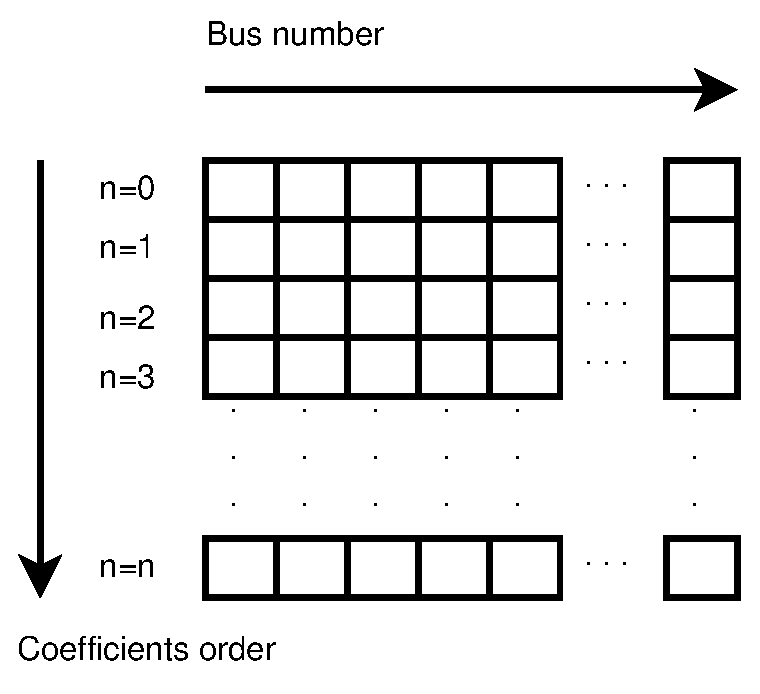
\includegraphics[width=0.4\linewidth]{CoefficientsStructure.eps}
	\caption{Structure of the coefficients}
	\label{fig:CoefficientsStructure}
\end{figure}

\subsection{Padè approximation}

The equation \ref{eq:McLaurinV} provides us with an expression to obtain the voltage from the coefficients, knowing that for $\alpha=1$ we get the final voltage results. So, why do we need any further operation?, and what is this Padè thing?

Well, it is true that the equation \ref{eq:McLaurinV} provides an approximation of the voltage by means of a series (this is similar to a Taylor approximation), but in practice, the approximation might provide a wrong value for a given number of coefficients. The Padè approximation accelerates the convergence of any given series, so that you get a more accurate result with less coefficients. This means that for the same series of voltage coefficients, using the equation \ref{eq:McLaurinV} could give a completely wrong result, whereas by applying Padè to those coefficients one could obtain a fairly accurate result.

The Padè approximation is a rational approximation of a function. In our case the function is $\textbf{V}(\alpha)$, represented by the coefficients structure $\textbf{V}$. The approximation is valid over a small domain of the function, in our case the domain is $\alpha=[0,1]$. The method requires the function to be continuous and differentiable for $\alpha=0$. Hence the Cauchy-Riemann condition. And yes, our function meets this condition, we tested it before.

GridCal implements two algorithms that perform the Padè approximation; The Padè canonical algorithm, and Wynn's Padè approximation.

\subsubsection{Padè approximation algorithm}

The canonical Padè algorithm for our problem is described by:

\begin{equation}
Voltage\_value\_approximation = \frac{P_N(\alpha)}{Q_M(\alpha)} \quad \forall \alpha \in [0,1]
\label{eq:pade_apprx}
\end{equation}

Here $N=M=n/2$, where $n$ is the number of available voltage coefficients, which has to be an even number to be exactly divisible by $2$. $P$ and $Q$ are polynomials which coefficients $p_i$ and $q_i$ must be computed. It turns out that if we make the first term of $Q_M(\alpha)$ be $q_0=1$, the function to be approximated is given by the McLaurin expression (What a happy coincidence!)
\begin{equation}
P_N(\alpha) = p_0 + p_1\alpha + p_2\alpha^2 + ... + p_N\alpha^N
\end{equation}

\begin{equation}
Q_M(\alpha) = 1 + q_1\alpha + q_2\alpha^2 + ... + q_M\alpha^M
\end{equation}



The problem now boils down to find the coefficients $q_i$ and $p_i$. This is done by solving two systems of equations. The first one to find $q_i$ which does not depend on $p_i$, and the second one to get $p_i$ which does depend on $q_i$.

\textbf{First linear system}: The only unknowns are the $q_i$ coefficients.

\begin{equation}
\begin{matrix}
q_M V_{N-M+1} + q_{M-1}V_{N-M+2}+...+q_1V_N = 0\\
q_M V_{N-M+2} + q_{M-1}V_{N-M+3}+...+q_1V_{N+1} = 0\\
...\\
q_M V_{N} + q_{M-1}V_{N+1}+...+q_1V_{N+M+1} + V_{N+M} = 0\\
\end{matrix}
\end{equation}

\textbf{Second linear System}: The only unknowns are the $p_i$ coefficients.
\begin{equation}
\begin{matrix}
V_0 - p_0=0\\
q_1V_0 + V_1  p_1=0\\
q_2V_0 + q_1V_1+V_2-p_2=0\\
q_3V_0 + q_2V_1 + q_1V_2 + V_3 - p_3 = 0\\
...\\
q_MV_{N-M} + q_{M-1}V_{N-M+1} + ... + +V_N - p_N=0
\end{matrix}
\end{equation}

Once the coefficients are there, you would have defined completely the polynomials $P_N(\alpha)$ and $Q_M(\alpha)$, and it is only a matter of evaluating the equation \ref{eq:pade_apprx} for $\alpha=1$.\newline


This process is done for every column of coefficients $\textbf{V}=\{V_0, V_1,V_2,V_3, ...,V_n\}$ of the structure depicted in the figure \ref{fig:CoefficientsStructure}. This means that we have to perform a Padè approximation for every node, using the one columns of the voltage coefficients per Padé approximation.

\subsubsection{Wynn's Padè approximation algorithm}

Wynn published a paper in 1969 where he proposed a simple calculation method to obtain the Padè approximation. This method is based on a table. Weniger in 1989 publishes his thesis where a faster version of Wynn's algorithm is provided in Fortran code. 

That very Fortran piece of code has been translated into Python and included in GridCal.

One of the advantages of this method over the canonical Padè approximation implementation is that it can be used for every iteration. In the beginning I thought it would be faster but it turns out that it is not faster since the amount of computation increases with the number of coefficients, whereas with the canonical implementation the order of the matrices does not grow dramatically and it is executed the half of the times.

On top of that my experience shows that the canonical implementation provides a more consistent convergence.

Anyway, both implementations are there to be used in the code.




\subsection{Formulation with PV nodes}

The section \ref{helm_fundamentals} introduces the canonical HELM algorithm. That algorithm does not include the formulation of PV nodes.
Other articles published on the subject feature PV formulations that work more or less to some degree. The formulation below is a formulation corrected by myself from a formulation contained here \cite{liu2017online}, which does not work as published, hence the correction.



\subsubsection{Embedding}

The following embedding equations are proposed instead of the canonical HELM equations from section \ref{helm_fundamentals}.

For Slack nodes:
\begin{equation}
V(\alpha) = V^{SP} \quad \forall \alpha=0
\end{equation}

For PQ nodes:
\begin{equation}
\left\{
\begin{array}{ll}
\textbf{Y} \times \textbf{V}(\alpha) = 0 \quad \quad \quad \quad \forall \alpha=0\\
\mathlarger{\textbf{Y} \times \textbf{V}(\alpha) = \frac{\alpha \textbf{S}}{\textbf{V}^*(\alpha^*)}} \quad \forall \alpha>0
\end{array}
\right.
\end{equation}

For PV nodes:

\begin{equation}
\left\{
\begin{array}{ll}
\mathlarger{\textbf{Y} \times \textbf{V}(\alpha) = \frac{ \textbf{S}}{\textbf{V}^*(\alpha^*)}} \quad \forall \alpha=0\\
\mathlarger{\textbf{Y} \times \textbf{V}(\alpha) = \frac{ \textbf{S} - j \textbf{Q}(\alpha)}{\textbf{V}^*(\alpha^*)}} \quad \forall \alpha>0
\end{array}
\right.
\end{equation}

\begin{equation}
\left\{
\begin{array}{ll}
V(\alpha)V^*(\alpha^*) = |V_0|^2\quad \quad \quad \quad \forall \alpha=0\\
V(\alpha)V^*(\alpha^*) = |V_0|^2 + (|V^{SP}|^2-|V_0|^2) \quad \forall \alpha>0
\end{array}
\right.
\end{equation}




This embedding translates into the following formulation:

\subsubsection{Step 1}

The formulas are adapted to exemplify a 3-bus system where the bus1 is a slack, the bus 2 is PV and the bus 3 is PQ. This follows the example of the Appendix A of \cite{liu2017online}.
\newline\newline
Compute the initial no-load solution ($n=0$):

\begin{equation}
\begin{bmatrix}
1 & 0 & 0 & 0 & 0 & 0\\
0 & 1 & 0 & 0 & 0 & 0\\
G_{21} & -B_{21} & G_{22} & -B_{22} & G_{23} & -B_{23}\\
B_{21} & G_{21}  & B_{22} & G_{22}  & B_{23} & G_{23}\\
G_{31} & -B_{31} & G_{32} & -B_{32} & G_{33} & -B_{33}\\
B_{31} & G_{31}  & B_{32} & G_{32}  & B_{33} & G_{33}\\
\end{bmatrix}
\times
\begin{bmatrix}
V[n]_{re, 1}\\
V[n]_{im, 1}\\
V[n]_{re, 2}\\
V[n]_{im, 2}\\
V[n]_{re, 3}\\
V[n]_{im, 3}\\
\end{bmatrix}
=
\begin{bmatrix}
V^{SP}_{re, 1}\\
V^{SP}_{im, 1}\\
0\\
0\\
0\\
0\\
\end{bmatrix}
\quad \forall n = 0
\end{equation}

Form the solution vector $\textbf{V}[n]$ you can compute the buses calculated power and then get the reactive power at the PV nodes to initialize $\textbf{Q}[0]$:

\begin{equation}
\textbf{S} = \textbf{V}[0] \cdot (\textbf{Y}_{bus} \times \textbf{V}[0])^*
\label{Scalc}
\end{equation}

\begin{equation}
\textbf{Q}_i[0] = imag(\textbf{S}_{i}) \quad \forall i \in PV
\end{equation}

The initial inverse voltage coefficients $\textbf{W}[0]$ are obtained by:

\begin{equation}
W_i[0] = \frac{1}{V_i[0]}  \quad \forall i \in N
\end{equation}

This step is entirely equivalent to find the no load solution using the Z-Matrix reduction.

\subsubsection{Step 2}

Construct the system of equations to solve the coefficients of order greater than zero ($n>0$). Note that the matrix is the same as constructed for the previous step, but adding a column and a row for each PV node to account for the reactive power coefficients. In our 3-bus example, there is only one PV node, so we add only one column and one row.

\begin{equation}
\begin{bmatrix}
1 & 0 & 0 & 0 & 0 & 0 & 0\\
0 & 1 & 0 & 0 & 0 & 0 & 0\\
G_{21} & -B_{21} & G_{22} & -B_{22} & G_{23} & -B_{23} & W[0]_{im}\\
B_{21} & G_{21}  & B_{22} & G_{22}  & B_{23} & G_{23} & W[0]_{re}\\
G_{31} & -B_{31} & G_{32} & -B_{32} & G_{33} & -B_{33} & 0\\
B_{31} & G_{31}  & B_{32} & G_{32}  & B_{33} & G_{33} & 0\\
0 & 0 & V[0]_{re} & V[0]_{im} & 0 & 0 & 0\\
\end{bmatrix}
\times
\begin{bmatrix}
V[n]_{re, 1}\\
V[n]_{im, 1}\\
V[n]_{re, 2}\\
V[n]_{im, 2}\\
V[n]_{re, 3}\\
V[n]_{im, 3}\\
Q_2[n]\\
\end{bmatrix}
=
\begin{bmatrix}
0\\
0\\
f2_{re}\\
f2_{im}\\
f1_{re}\\
f1_{im}\\
\epsilon[n]\\
\end{bmatrix}
\quad \forall n > 0
\label{lin_sys_2}
\end{equation}

Where:

\begin{equation}
f1 = S^*_i \cdot W^*_i[n-1] \quad \forall i \in PQ
\end{equation}

\begin{equation}
f2 = P_i \cdot W^*_i[n-1] + conv(n, Q_i, W^*_i) \quad \forall i \in PV
\end{equation}

\begin{equation}
\epsilon[n] = \delta_{n1} \cdot \frac{1}{2} \left(|V_i^SP|^2 - |V_i[0]|^2\right) - \frac{1}{2} conv(n, V_i, V_i^*)  \quad \forall i \in PV, n > 0
\end{equation}

The convolution $conv$ is defined as:

\begin{equation}
conv(n, A, B) = \sum_{m=0}^{n-1} A[m] \cdot B[n-m]
\end{equation}

The system matrix ($A_{sys}$) is the same for all the orders of $n>0$, therefore we only build it once, and we factorize it to solve the subsequent coefficients.

After the voltages $\textbf{V}[n]$ and the reactive power at the PV nodes $Q[n]$ is obtained solving the linear system (eq \ref{lin_sys_2}), we must solve the inverse voltage coefficients of order $n$ for all the buses:

\begin{equation}
W_i[n] = \frac{- \mathlarger{\sum_{m=0}^{n}W_i[m] \cdot V_i[n-m]} }{V_i[0]} \quad  \forall i \in N, n>0
\end{equation}


\subsubsection{Step 3}

Repeat step 2 until a sufficiently low error is achieved or a maximum number of iterations (coefficients).


The error is computed by comparing the calculated power $\textbf{S}$ (eq \ref{Scalc}) with the specified power injections $\textbf{S}^{SP}$:

\begin{equation}
mismatch = \textbf{S} - \textbf{S}^{SP}
\end{equation}

\begin{equation}
error = |mismatch|_\infty = max(abs(mismatch))
\end{equation}

\newpage
\section{Post power flow (loading and losses)}

As we have seen, the power flow routines compute the voltage at every bus of an island grid. However we do not get from those routines the "power flow" values, this is the power that flows through the branches of the grid. In this section I show how the \textit{post power flow} values are computed. \newline


First we compute the branches per unit currents:

\begin{equation}
{\textbf{I}_f = \textbf{Y}_f \times \textbf{V}}
\end{equation}

\begin{equation}
{\textbf{I}_t = \textbf{Y}_t \times \textbf{V}}
\end{equation}


These are matrix-vector multiplications. The result is the per unit currents flowing through a branch seen from the \textit{from} bus or from the \textit{to} bus.


Then we compute the power values:

\begin{equation}
{\textbf{S}_f = \textbf{V}_f \cdot \textbf{I}_f^*}
\end{equation}

\begin{equation}
{\textbf{S}_t = \textbf{V}_t \cdot \textbf{I}_t^*}
\end{equation}

These are element-wise multiplications, resulting in the per unit power flowing through a branch seen from the \textit{from} bus or from the \textit{to} bus.

Now we can compute the losses in MVA as:

\begin{equation}
{\textbf{losses} = |\textbf{S}_f - \textbf{S}_t| \cdot Sbase}
\end{equation}

And also the branches loading in per unit as:
\begin{equation}
{\textbf{loading} = \frac{max(|\textbf{S}_f|, |\textbf{S}_t|) \cdot Sbase}{ \textbf{rate}}}
\end{equation}

The variables are:

\begin{itemize}
	\item $\textbf{Y}_f, \textbf{Y}_t$: \textit{From} and \textit{To} bus-branch admittance matrices, see section \ref{admitances_section}.
	\item $\textbf{I}_f$: Array of currents at the \textit{from} buses in p.u.
	\item $\textbf{I}_t$: Array of currents at the \textit{to} buses in p.u.
	\item $\textbf{S}_f$: Array of powers at the \textit{from} buses in p.u.
	\item $\textbf{S}_t$: Array of powers at the \textit{to} buses in p.u.
	\item $\textbf{V}_f$: Array of voltages at the \textit{from} buses in p.u.
	\item $\textbf{V}_t$: Array of voltages at the \textit{to} buses in p.u.
	\item $\textbf{rate}$: Array of branch ratings in MVA.
\end{itemize}



\chapterimage{chapterhdr1.jpg} % Chapter heading image
\chapter{Short circuit}

%I = zeros(n, dtype=complex)
%I[bus_idx] = -1 * Vbus[bus_idx] / (Zbus[bus_idx, bus_idx] + Zf)
%
%incV = Zbus.dot(I)
%
%V = Vbus + incV

\section{3-phase short circuit}

First, declare an array of zeros of size equal to the number of nodes in the circuit.

$$
\textbf{I} = \{0, 0, 0, 0, ..., 0\}
$$

Then, compute the short circuit current at the selected bus $i$ and assign that value in the $i^{th}$ position of the array $\textbf{I}$.
\begin{equation}
\textbf{I}_i = - \frac{\textbf{V}_{pre-failure, i}}{\textbf{Z}_{i, i} + z_f}
\end{equation}

Then, compute the voltage increment for all the circuit nodes as:
\begin{equation}
\Delta \textbf{V} = \textbf{Z} \times \textbf{I}
\end{equation}

Finally, define the voltage at all the nodes as:

\begin{equation}
\textbf{V}_{post-failure} = \textbf{V}_{pre-failure} + \Delta \textbf{ V}
\end{equation}

Magnitudes:
\begin{itemize}
	\item $\textbf{I}$: Array of fault currents at the system nodes.
	\item $\textbf{V}_{pre-failure}$: Array of system voltages prior to the failure. This is obtained from the power flow study.
	\item $z_f$: Impedance of the failure itself. This is a given value, although you can set it to zero if you don't know.
	\item $\textbf{Z}$: system impedance matrix. Obtained as the inverse of the complete system admittance matrix.
	
\end{itemize}

%----------------------------------------------------------------------------------------
%	CHAPTER 4
%----------------------------------------------------------------------------------------

\chapterimage{chapterhdr1.jpg} % Chapter heading image
\chapter{Graphical User Interface}

\begin{figure}[h!]
	\centering
	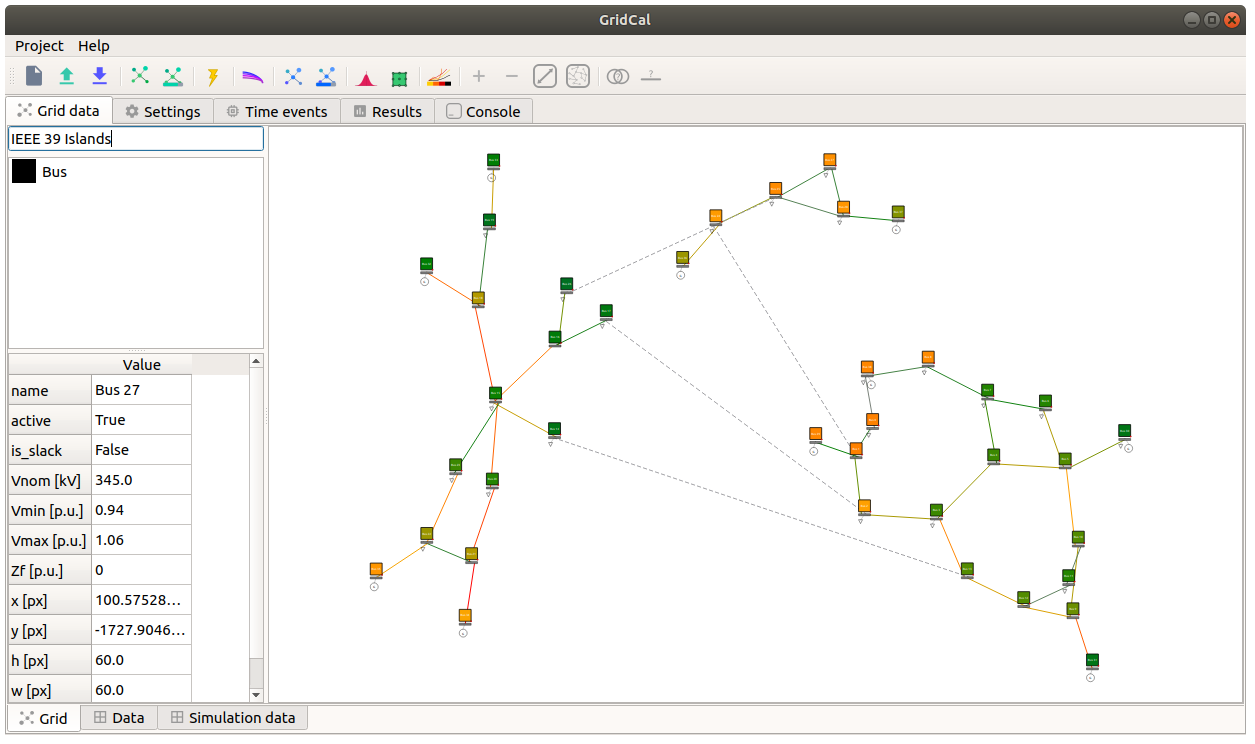
\includegraphics[width=0.98\linewidth]{GridData.png}
	\caption{GridCal user interface representing the IEEE 39 bus grid split in three islands.}
	\label{fig:main_gui}
\end{figure}

% ----------------------------------------------------------------------------------------
% 	BIBLIOGRAPHY
% ----------------------------------------------------------------------------------------
%\chapter*{Bibliography}
\bibliographystyle{unsrt}
\bibliography{bibliography}

\end{document}